%%%%%%%%%%%%%%%%%%%%%%%%%%%%%%%%%%%%%%%%%%%%%%%%%%%%%%%%%%%%%%%%%%%%%%%%%%%%%%%%
% AMS Beamer series / Bologna FC / Template
% Andrea Omicini
% Alma Mater Studiorum - Università di Bologna
% mailto:andrea.omicini@unibo.it
%%%%%%%%%%%%%%%%%%%%%%%%%%%%%%%%%%%%%%%%%%%%%%%%%%%%%%%%%%%%%%%%%%%%%%%%%%%%%%%%
%\documentclass[handout]{beamer}\mode<handout>{\usetheme{default}}
%
\documentclass[presentation, 9pt]{beamer}\mode<presentation>{\usetheme{AMSBolognaFC}}
%\documentclass[handout]{beamer}\mode<handout>{\usetheme{AMSBolognaFC}}
%%%%%%%%%%%%%%%%%%%%%%%%%%%%%%%%%%%%%%%%%%%%%%%%%%%%%%%%%%%%%%%%%%%%%%%%%%%%%%%%
\usepackage[T1]{fontenc}
\usepackage{wasysym}
\usepackage{amsmath,blkarray}
\usepackage[minted,most]{tcolorbox}
\usepackage{centernot}
\usepackage{fontawesome}
\usepackage{fancyvrb}
\setminted[scala]{fontsize=\scriptsize,baselinestretch=1,obeytabs=true, tabsize=2}
\usepackage[ddmmyyyy]{datetime}
\renewcommand{\dateseparator}{}
%\renewcommand{\thefootnote}{\fnsymbol{footnote}}
\newcommand{\version}{1}
\usepackage[
	backend=biber,
	citestyle=authoryear-icomp,
	maxcitenames=1,
	bibstyle=numeric]{biblatex}

	\makeatletter
	\setbeamercovered{transparent}
\addbibresource{biblio.bib}
%%%%%%%%%%%%%%%%%%%%%%%%%%%%%%%%%%%%%%%%%%%%%%%%%%%%%%%%%%%%%%%%%%%%%%%%%%%%%%%%
\title[MacroSwarm]
{MacroSwarm \\ Field-based Compositional Framework for Swarm Programming}
%
%subtitle[How to build applications that span in different platforms]
%{How to build applications that span in different platforms}
%
\author[\sspeaker{Aguzzi}]
{\speaker{Gianluca Aguzzi} \href{mailto:gianluca.aguzzi@unibo.it}{gianluca.aguzzi@unibo.it}\\
\otherauthor{Roberto Casadei} \href{mailto:roby.casadei@unibo.it}{roby.casadei@unibo.it}\\
\otherauthor{Mirko Viroli} \href{mailto:mirko.viroli@unibo.it}{mirko.viroli@unibo.it}}
%
\institute[DISI, Univ.\ Bologna]
{Dipartimento di Informatica -- Scienza e Ingegneria (DISI)\\
\textsc{Alma Mater Studiorum} -- Universit{\`a} di Bologna \\[0.5cm]
\textbf{Talk @} \bold{COORDINATION 2023}

\vspace{0.2cm}
\fbox{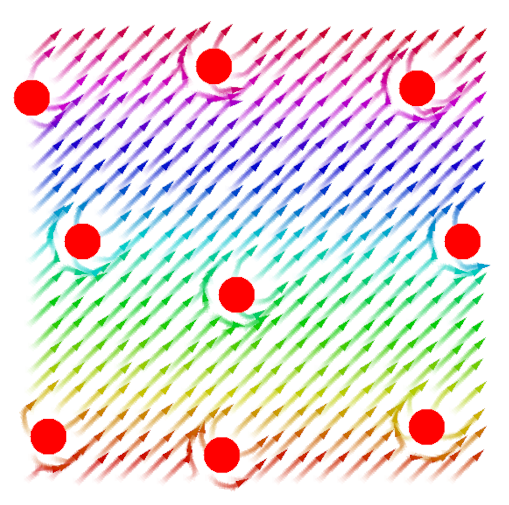
\includegraphics[width=0.2\textwidth]{img/obstacle-avoidance}}
\fbox{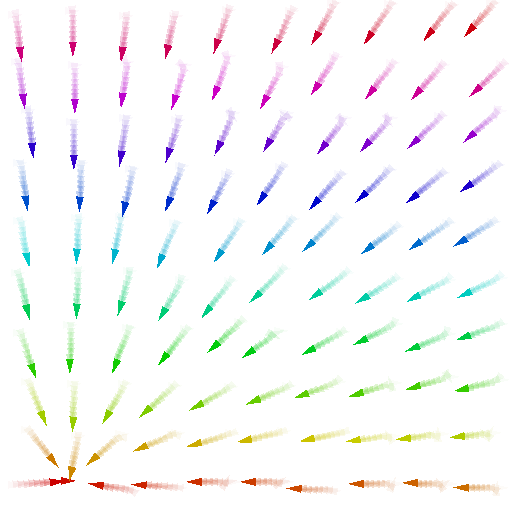
\includegraphics[width=0.2\textwidth]{img/towards-leader.png}}
\fbox{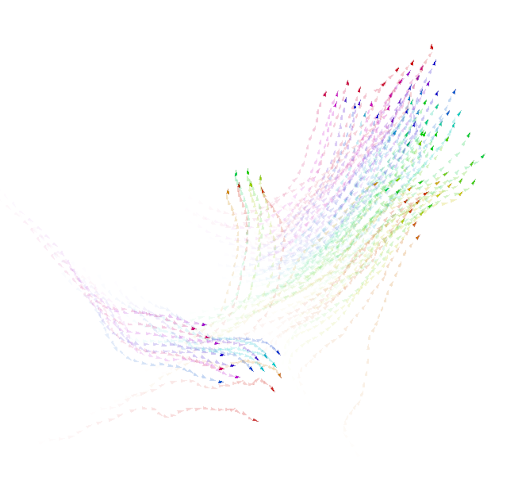
\includegraphics[width=0.2\textwidth]{img/flock.png}}
\fbox{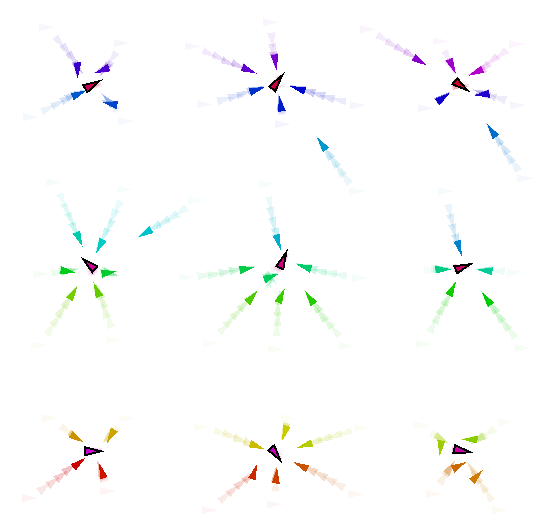
\includegraphics[width=0.2\textwidth]{img/team-formation.png}}}
%
\renewcommand{\dateseparator}{/}
\date[\today]{}
%
\AtBeginSection[]
{
  \begin{frame}
  \frametitle{Contents}
  \tableofcontents[currentsubsection, 
	sectionstyle=show/shaded, 
	subsectionstyle=show/shaded]
  \end{frame}
}
\AtBeginSubsection[]
{
  \begin{frame}
  \frametitle{Contents}
  \tableofcontents[currentsubsection, 
	sectionstyle=show/shaded, 
	subsectionstyle=show/shaded]
  \end{frame}
}
%%%%%%%%%%%%%%%%%%%%%%%%%%%%%%%%%%%%%%%%%%%%%%%%%%%%%%%%%%%%%%%%%%%%%%%%%%%%%%%%
\begin{document}
%%%%%%%%%%%%%%%%%%%%%%%%%%%%%%%%%%%%%%%%%%%%%%%%%%%%%%%%%%%%%%%%%%%%%%%%%%%%%%%%

%/////////
\frame{\titlepage}
%/////////

%===============================================================================
\begin{frame}{Context}
\centering
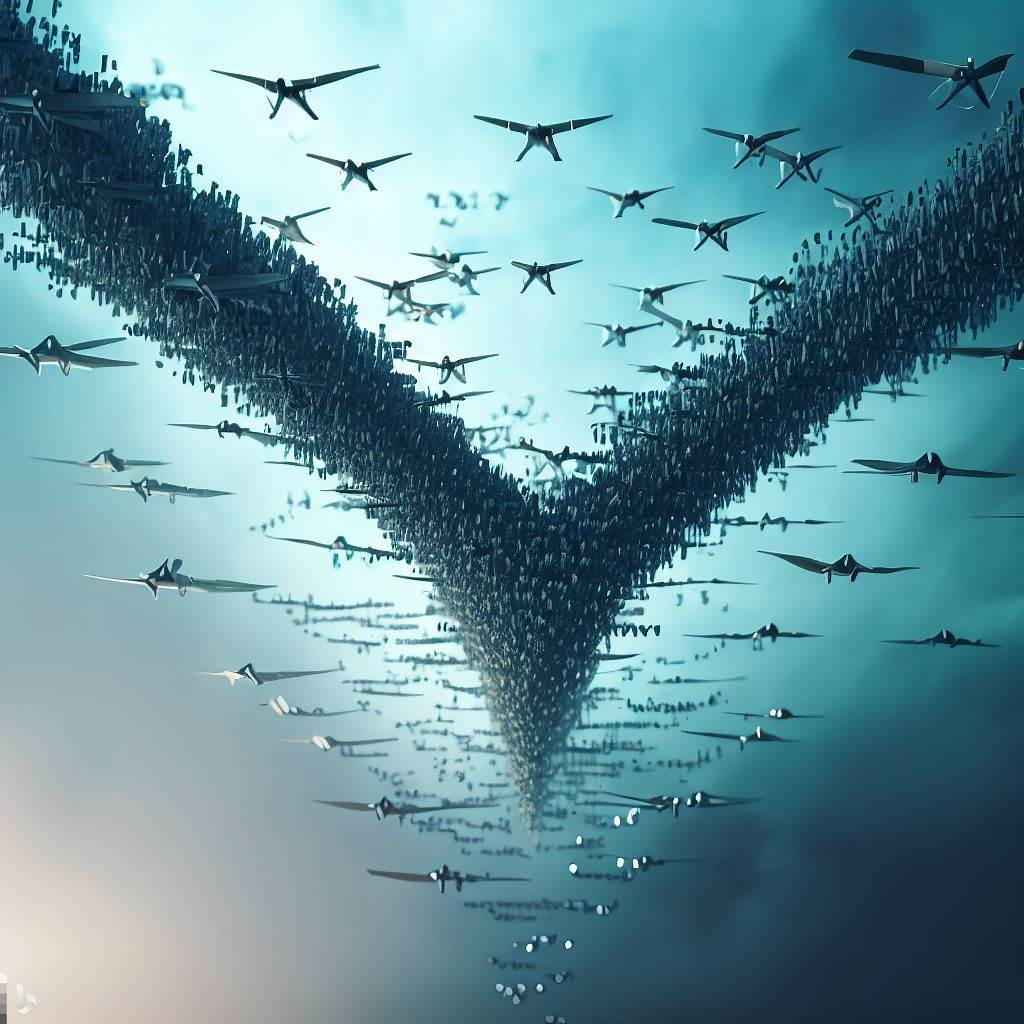
\includegraphics[width=0.55\textwidth]{img/flock.jpeg}
\\
\huge{\emph{Networked Mobile Nodes}} \faPlus \, \textbf{Collective Behaviors}
\end{frame}
\begin{frame}{Swarm Behaviors}
A \textbf{swarm behavior} is a \emph{collective} behavior that emerges from the \emph{local} interactions of a \emph{population} of \emph{autonomous} entities.
\begin{block}{Inspiration from Nature: Social Animals}
\begin{itemize}
	\item \emph{Ants} \faArrowRight \, \emph{foraging} and \emph{nest building}
	\item \emph{Fishes} \faArrowRight \, \emph{schooling}
	\item \emph{Bees} \faArrowRight \, \emph{swarming}
	\item \dots But now let us focus on \emph{engineering}! :)
\end{itemize}
\end{block}

\centering
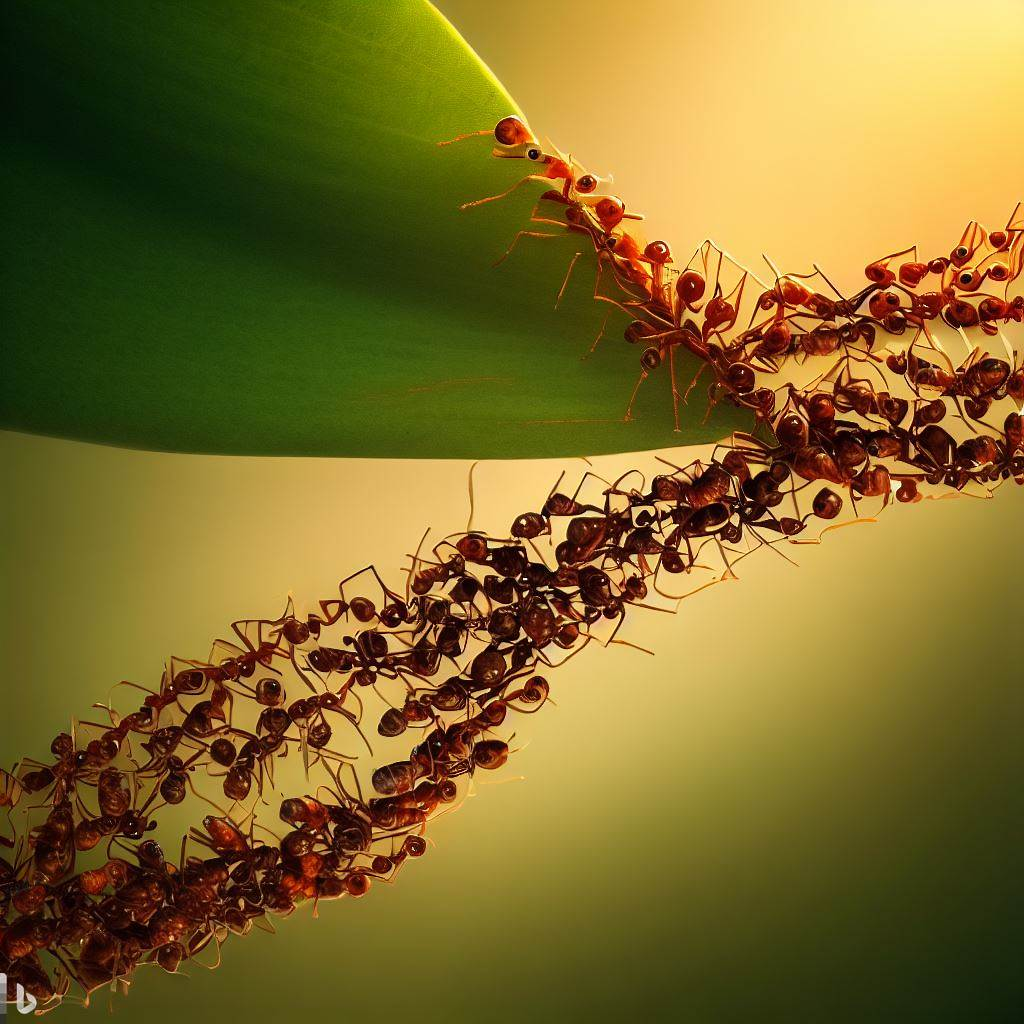
\includegraphics[width=0.15\textwidth]{img/ants.jpeg}
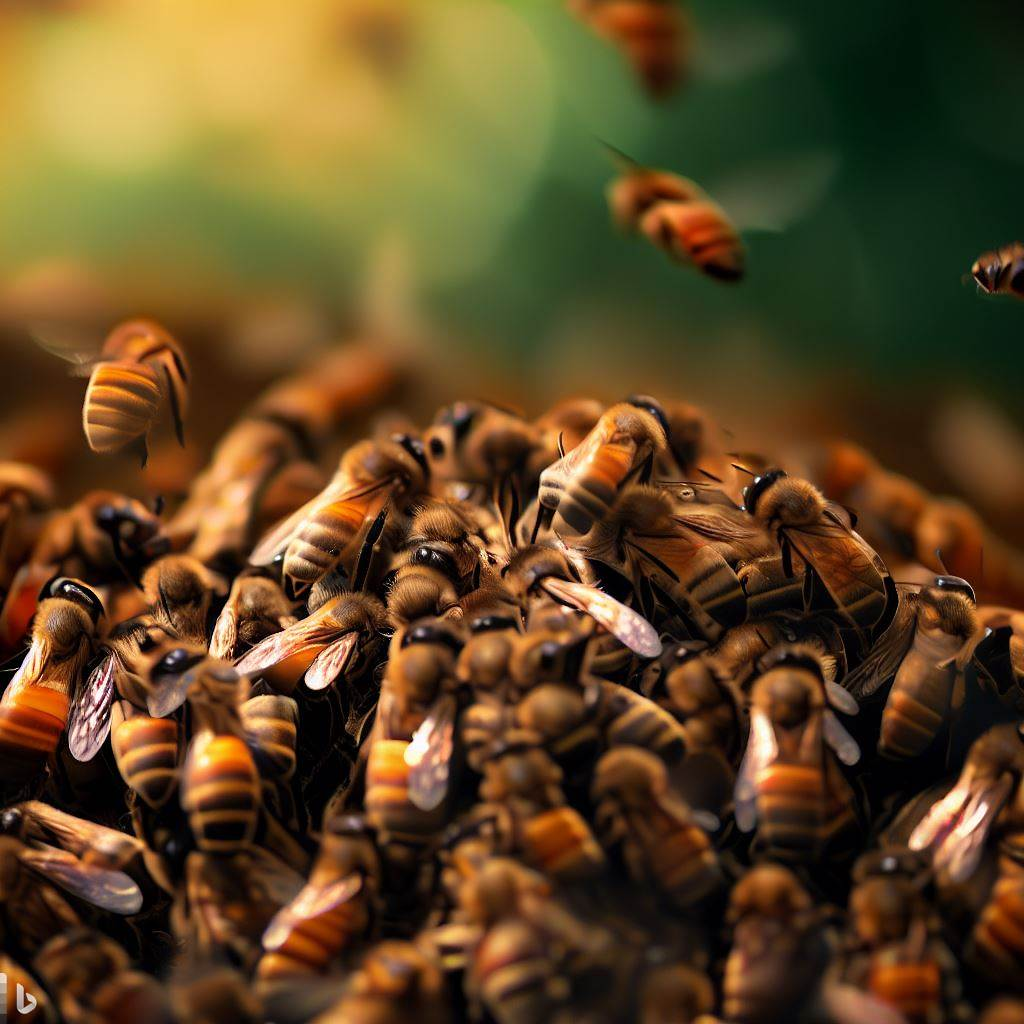
\includegraphics[width=0.15\textwidth]{img/bee.jpeg}
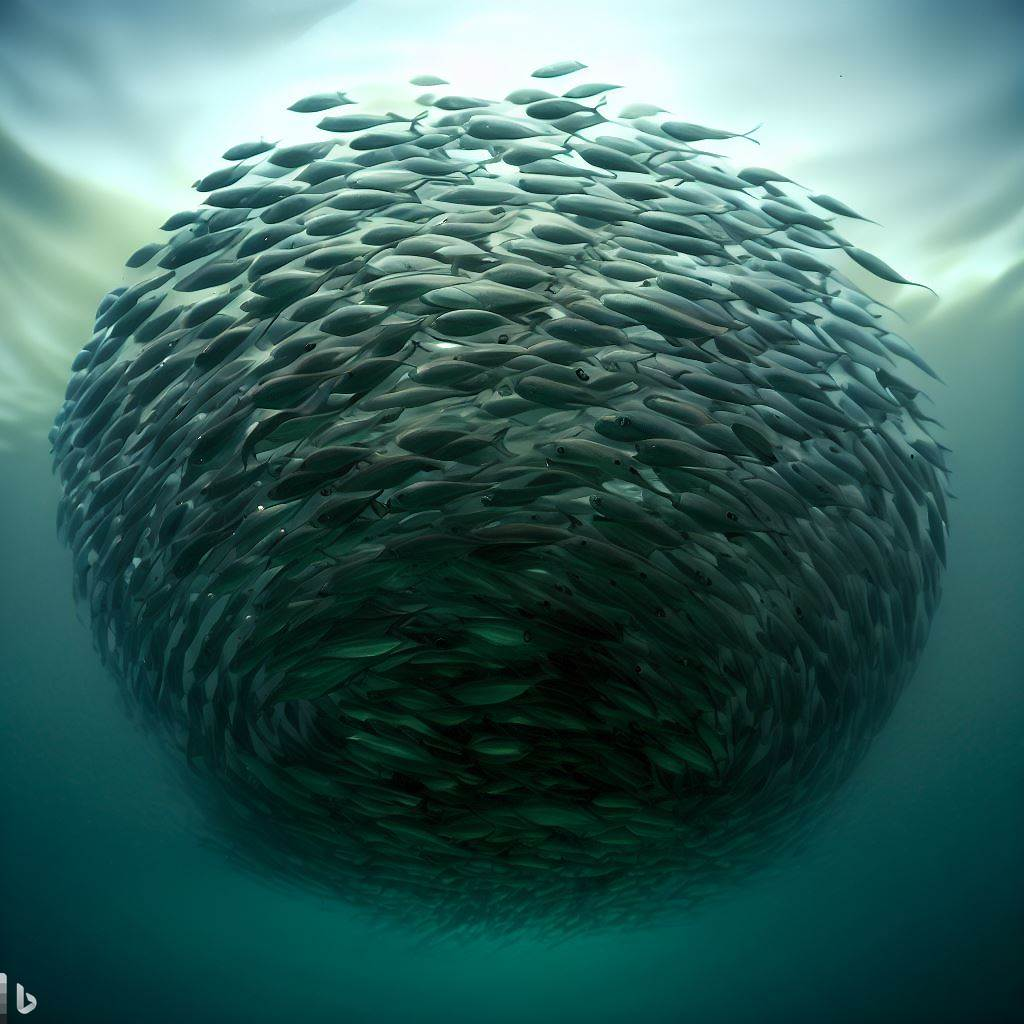
\includegraphics[width=0.15\textwidth]{img/fishes.jpeg}

\begin{alertblock}{In a nutshell}
\begin{itemize}
	\item \textbf{Emergent} \faArrowRight \, \emph{self-organisation} and \emph{self-adaptation}
	\item \textbf{Decentralized} \faArrowRight \, \emph{locality} and \emph{scalability}
	\item \textbf{Asynchronous} \faArrowRight \, \emph{robustness} and \emph{fault-tolerance}
\end{itemize}	
\end{alertblock}
\end{frame}
\begin{frame}{Swarm Behaviors: Taxonomy~\footnote{\fullcite{schranz2020swarm}}}
\begin{exampleblock}{Main classes}
	\begin{itemize}
		\item \textbf{Spatial Organization}: collective movements that lead to global spatial patterns
		\begin{itemize}
			\item Collective structures \faArrowRight \, functional to achieve certain goals
			\item \bold{Aggregation}, \bold{pattern formation}, \bold{self-assembly}, \bold{object clustering} 
		\end{itemize}
		\item \textbf{Navigation}: coordinated motion in order to reach a target/perform collective tasks
		\begin{itemize}
			\item \bold{Exploration}, \bold{motion}, \bold{transportation}, \bold{localization}
		\end{itemize}
		\item \textbf{Decision-making}: lead the system to reach a global decision %or consensus
		\begin{itemize}
			\item \bold{consensus}, \bold{task allocation}, \bold{group size regulation}, \bold{collective perception}, \dots
		\end{itemize}
	\end{itemize}
\end{exampleblock}

	\centering
	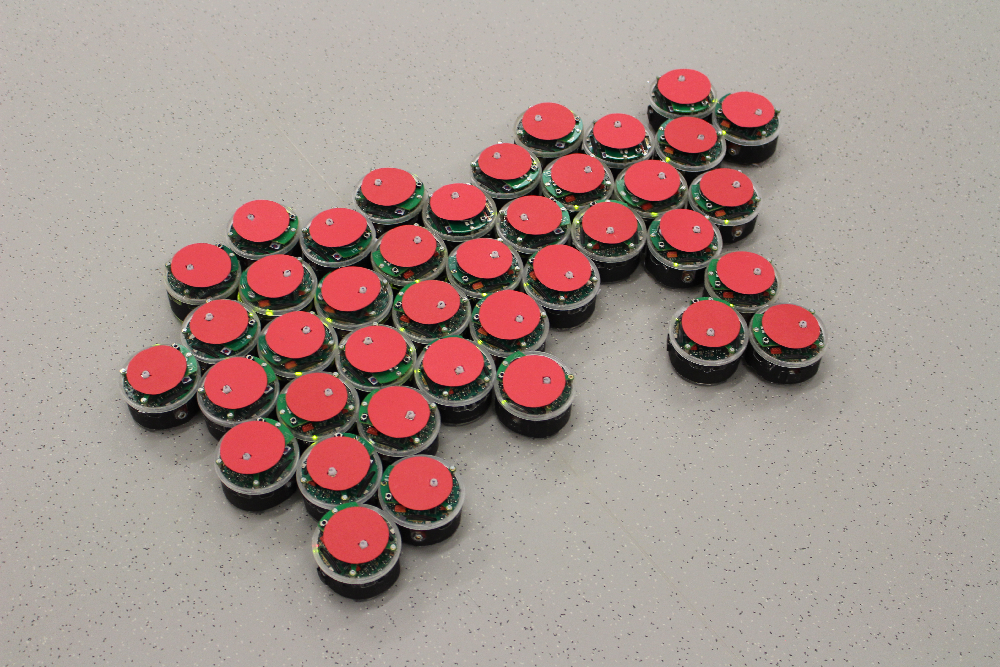
\includegraphics[height=1.6cm]{img/aggregation.jpg}
	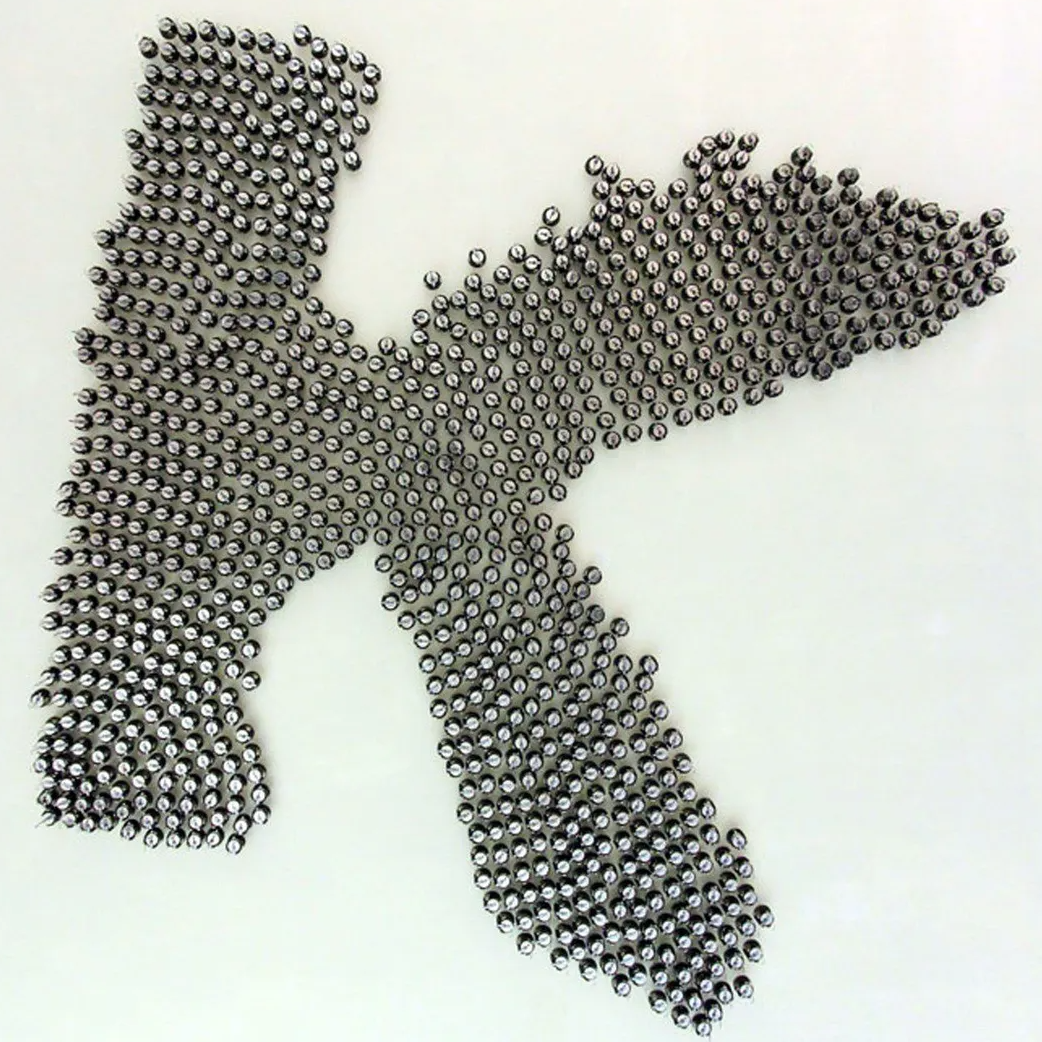
\includegraphics[height=1.6cm]{img/pattern-formation.png}
	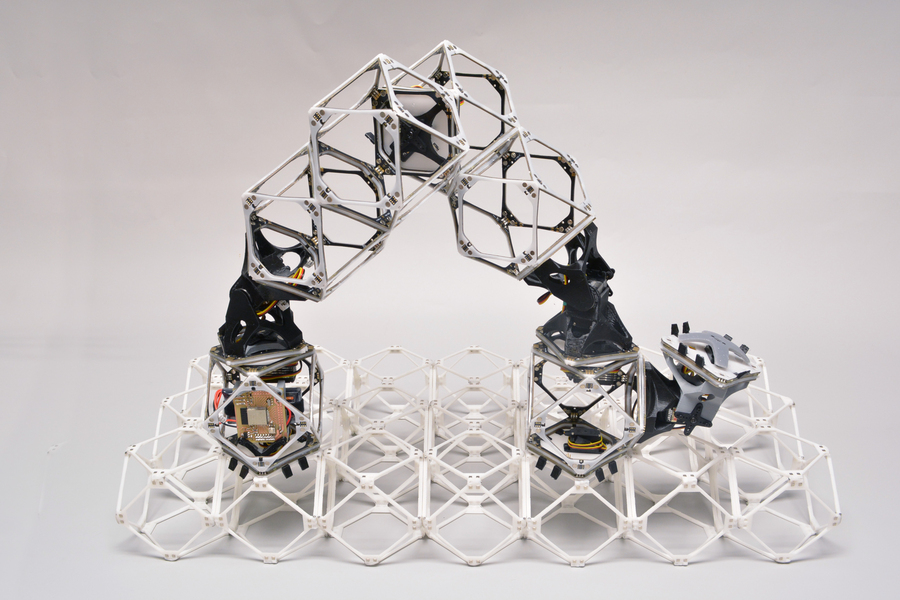
\includegraphics[height=1.6cm]{img/sefl-assembly.jpg}
	\\
	\centering
	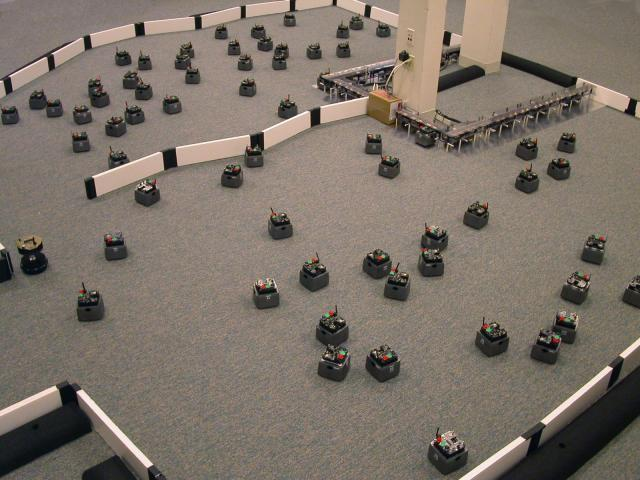
\includegraphics[height=1.6cm]{img/exploration.jpg}
	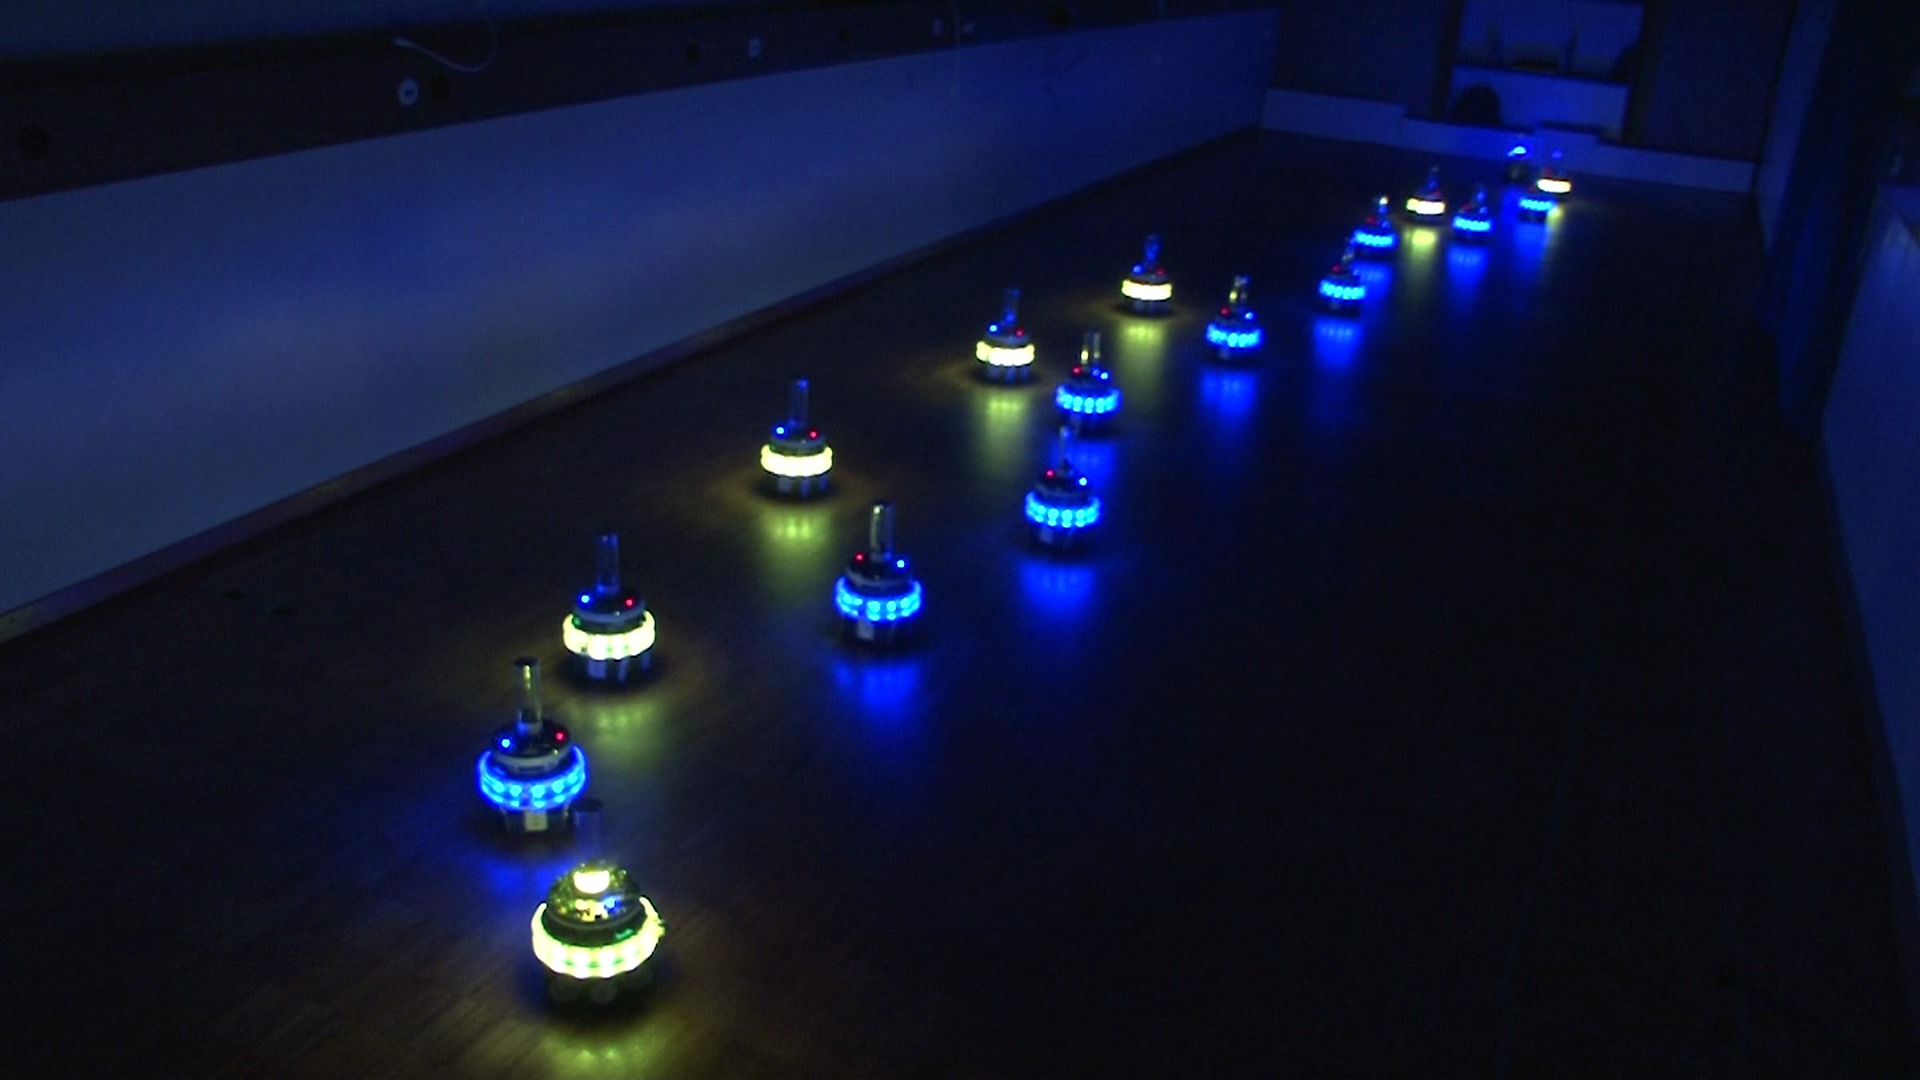
\includegraphics[height=1.6cm]{img/navigation.jpg}
	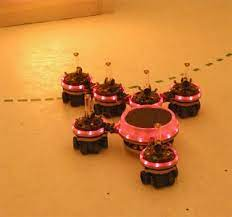
\includegraphics[height=1.6cm]{img/transportation.jpeg}
	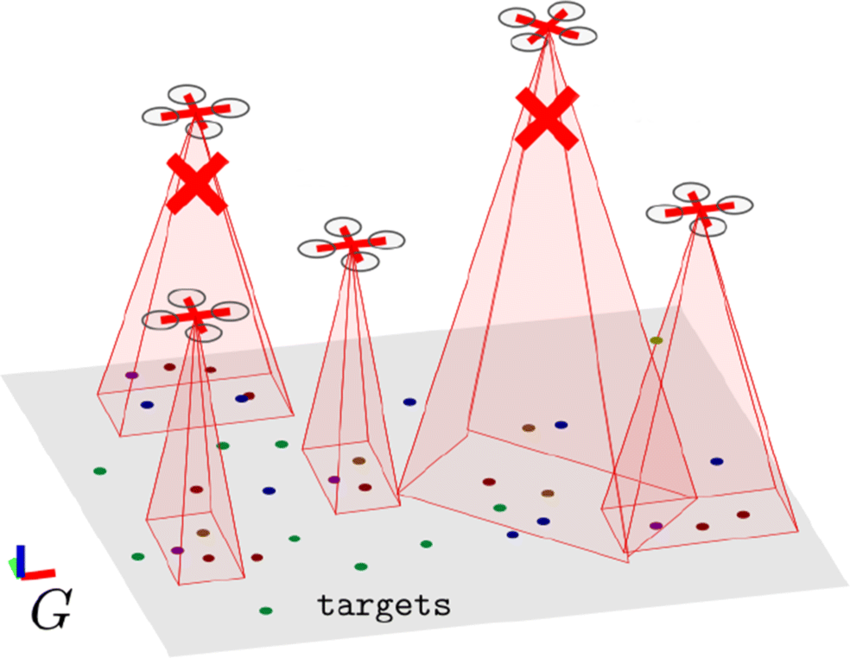
\includegraphics[height=1.6cm]{img/localization.png}

\end{frame}
\begin{frame}{Programming Swarm Behaviors -- Related Works}
	\begin{block}{Problems}
		\begin{itemize}
			\item How to express \emph{swarm behaviors}\footnote{\fullcite{Mone2013}}? \faArrowRight \, \emph{programming abstractions} 
			\begin{itemize}
				\item Move the viewpoint from \emph{individual} to \emph{collective} level \faArrowRight \, macro-programming 
			\end{itemize}
			\item \emph{Complexity} \faArrowRight \, \emph{collective} and \emph{individual} levels \faArrowRight \, \bold{programming the emergence}\footnote{\fullcite{varenne2015programming}}
			%\item \emph{Reusability} \faArrowRight \, \emph{compositionality} and \emph{modularity}
			\item \emph{Scalability} \faArrowRight \, avoiding \emph{centralized} and \emph{global} approaches
		\end{itemize}
	\end{block}
	\begin{alertblock}{Proposed solutions}
		\begin{itemize}
			\item Orchestration-based: centralized approaches for expressing swarm behaviours
			\begin{itemize}
				\item TeCoLa, Dolphin, PARoS
			\end{itemize}
			\item Choreograph-based: decentralized approaches for expressing swarm behaviours
			\begin{itemize}
				\item Buzz, Voltron, Meld
			\end{itemize}
		\end{itemize}
	\end{alertblock}
	\begin{block}{Limitations}
		\begin{itemize}
			\item Lack of modularity, no formal semantics, no practical implementation, \dots
		\end{itemize}
	\end{block}
\end{frame}
\begin{frame}{MacroSwarm}
\centering {
MacroSwarm\footnote{\url{https://github.com/AggregateComputing/experiment-2023-coordination-swarm-behaviour}} is based on a macro programming approach called \emph{Aggregate Computing}\footnote{\fullcite{viroli2018field}} (aka \emph{field-based coordination}) for programming swarm behaviors in a modular and scalable way.
}
\begin{alertblock}{Features}
	\begin{itemize}
		\item Cover the \emph{main classes} of swarm behaviors
		\item \emph{modular} and \emph{composable} behaviors
		\item purely functional transformations from input to actuation fields \faArrowRight \, easy to reason about
		\item Support several organization patterns \faArrowRight \, flock-based, leader-based, \dots
		\item Robust and scalable \faArrowRight \, \emph{decentralized} and \emph{asynchronous}
	\end{itemize}
\end{alertblock}
\end{frame}
\begin{frame}[allowframebreaks]{Aggregate Computing}
\begin{alertblock}{In a nutshell}
\begin{itemize}
	\item \emph{Computational fields} as first-class abstractions
	\item Programs as field transformations through \emph{field calculus} 
	\item Inspiration from \emph{co-fields} and \emph{artificial potential fields}
\end{itemize}
\end{alertblock}

\centering
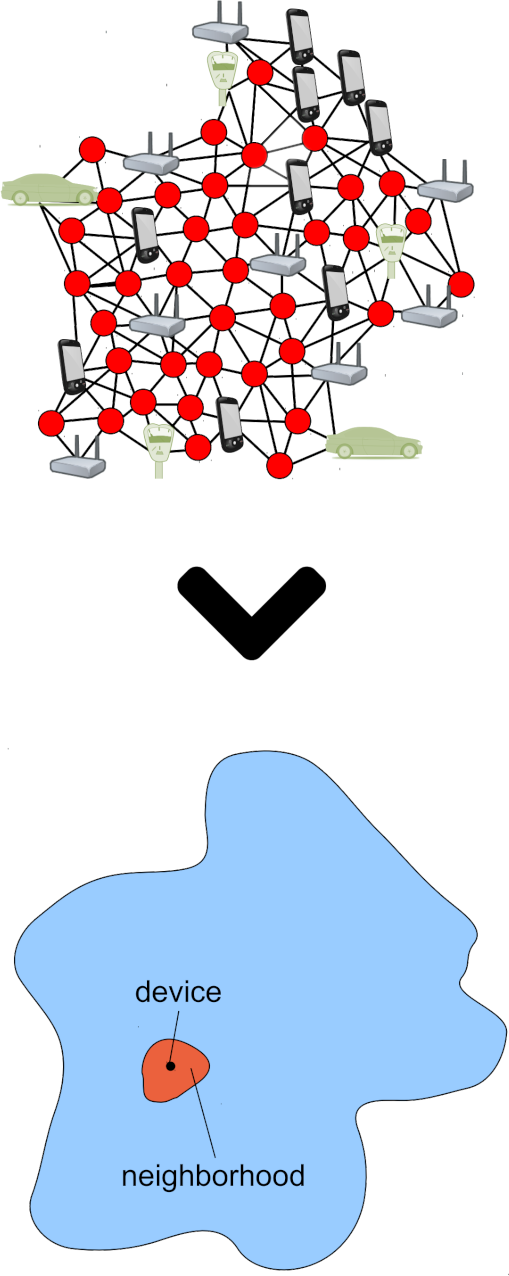
\includegraphics[height=5cm]{img/abstraction.png}
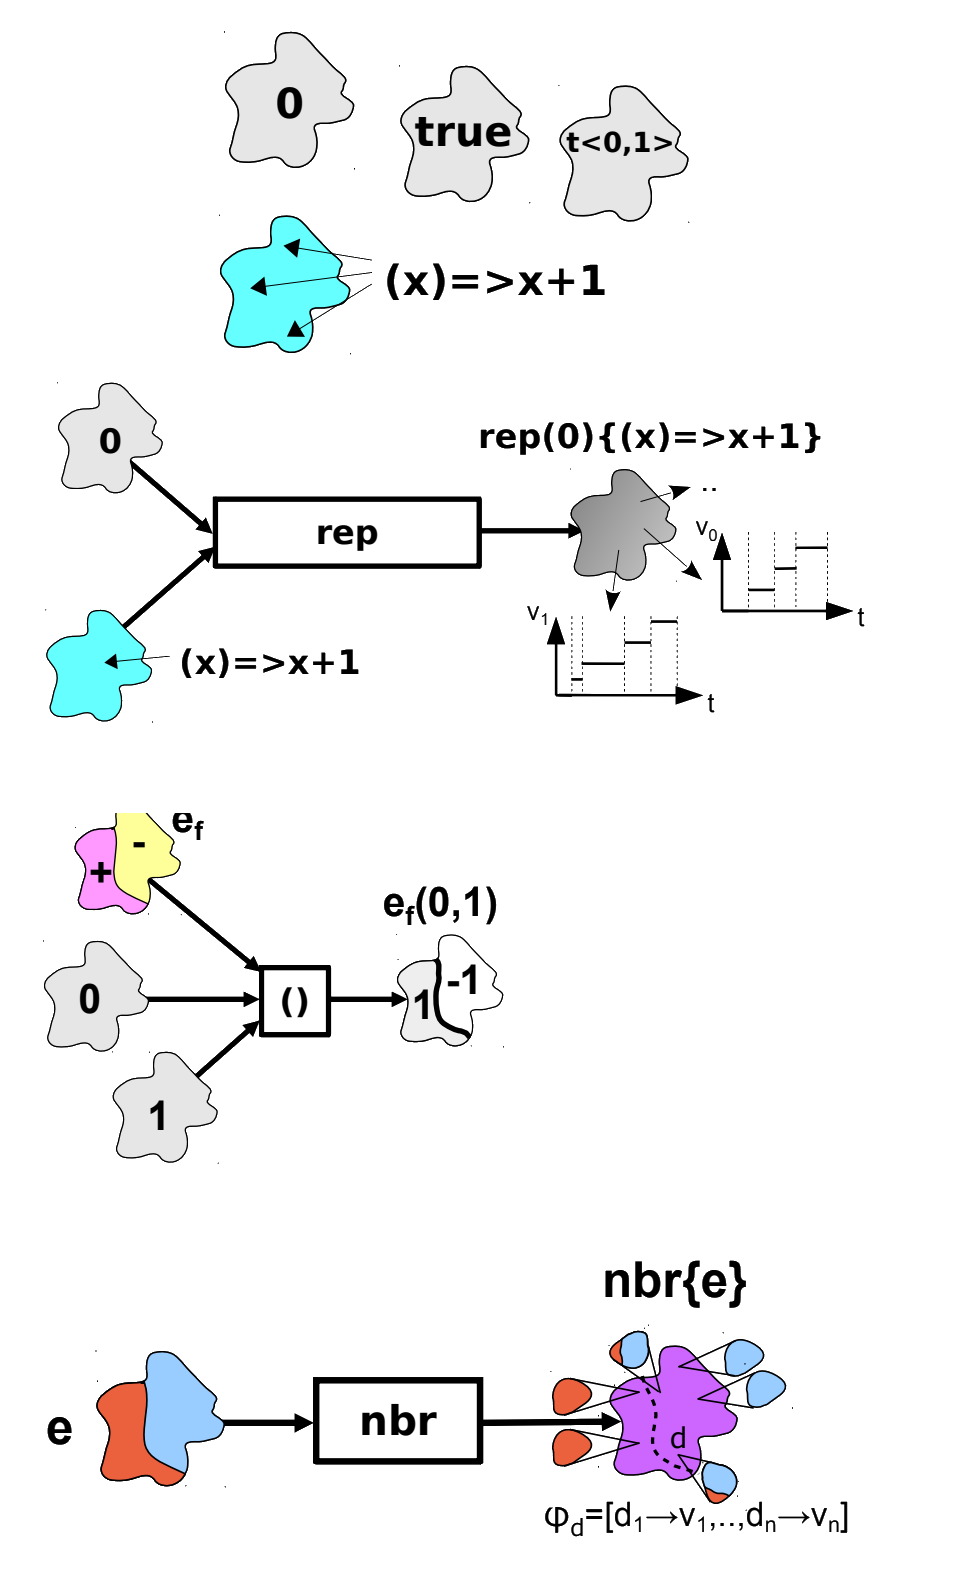
\includegraphics[height=5cm]{img/high-level-examples.png}
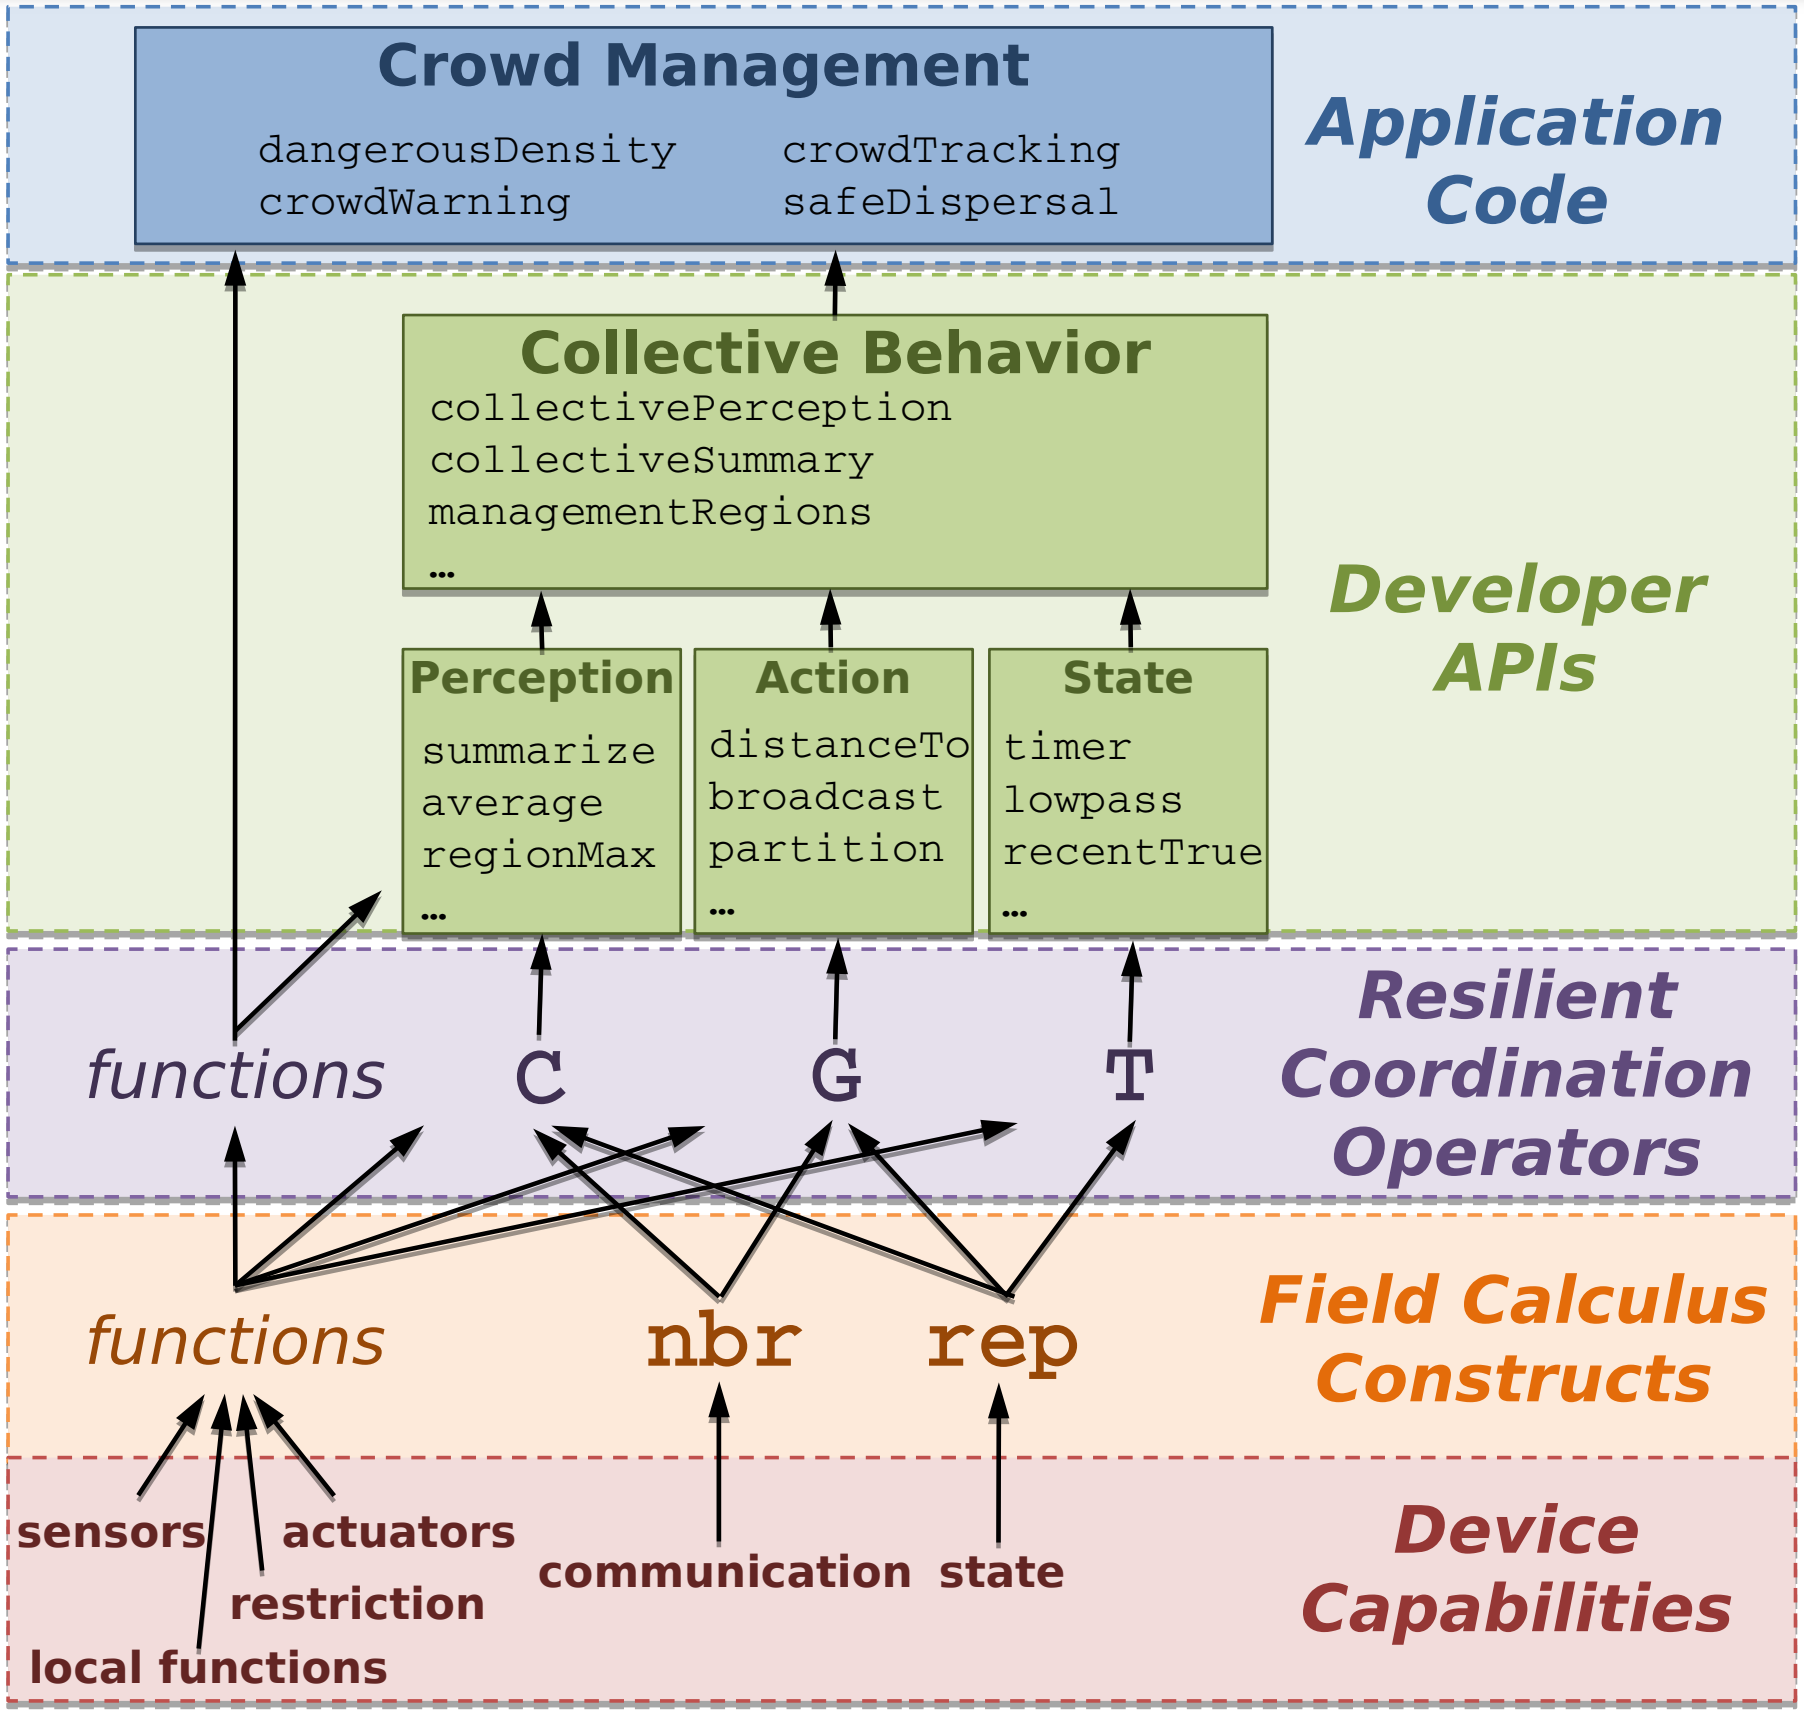
\includegraphics[height=5cm]{img/full-stack.png}
\begin{alertblock}{System model}
	\begin{itemize}
		\item An aggregate program is \emph{shared} by all the nodes
		\item Each node execute rounds iteratively and asynchronously:
		\begin{enumerate}
			\item \textbf{Context building}: collect information from the neighborhood and sensors
			\item \textbf{Program execution}: execute the aggregate program on the context
			\item \textbf{Export sharing}: share the export with the neighborhood
		\end{enumerate}
	\end{itemize}
\end{alertblock}
\begin{block}{Why}
\begin{itemize}
	\item \emph{Top-down behaviour-based design} \faArrowRight \, \emph{compositionality} and \emph{collective stance} of aggregate computing;
	\item \emph{Scalability} \faArrowRight \, fully decentralized and asynchronous
	\item \emph{Formal approach} \faArrowRight \, based on the field calculus
		
	\item \emph{Pragmatism} \faArrowRight \, witnessed by open-source, maintained, concrete software artifacts like the ScaFi DSL, Alchemist and {\sc{}ScaFi-Web}
	\item \emph{Operational flexibility} \faArrowRight \, supporting different architectural styles and execution policies.
\end{itemize}

\end{block}

\end{frame}

\begin{frame}{Architecture}
\centering
\fbox{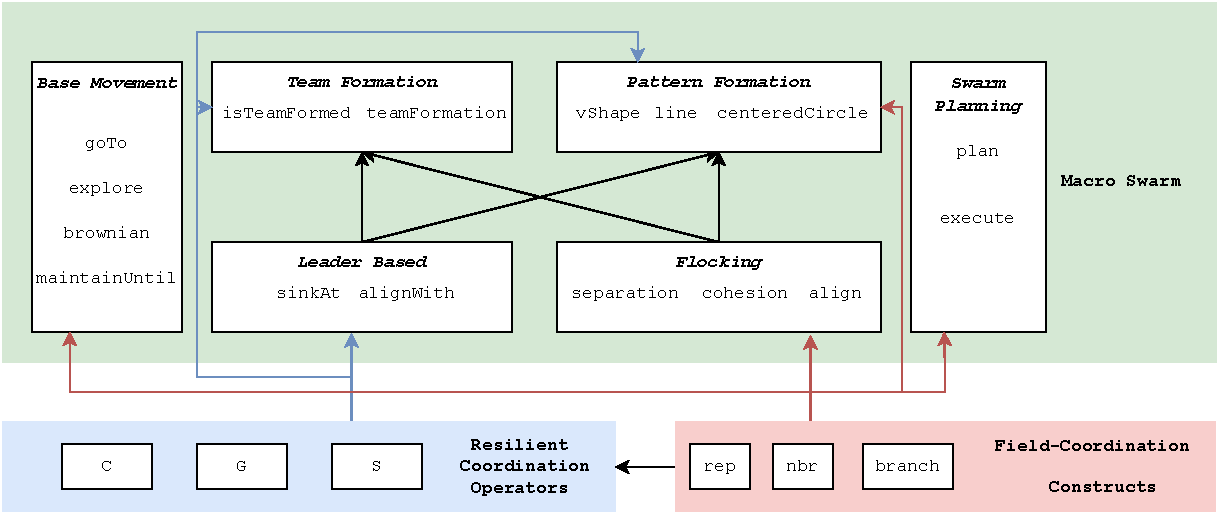
\includegraphics[width=0.98\textwidth]{img/architecture.drawio.pdf}}
\end{frame}
\begin{frame}[fragile]{API Overview: Basic Movements}
\centering
Control the movement of the individual agents within the swarm
\begin{columns}
	\begin{column}[t]{0.3\textwidth}
		\begin{exampleblock}{Constant movement}
		\begin{minted}{scala}
Velocity2D(0, 1)
		\end{minted}
		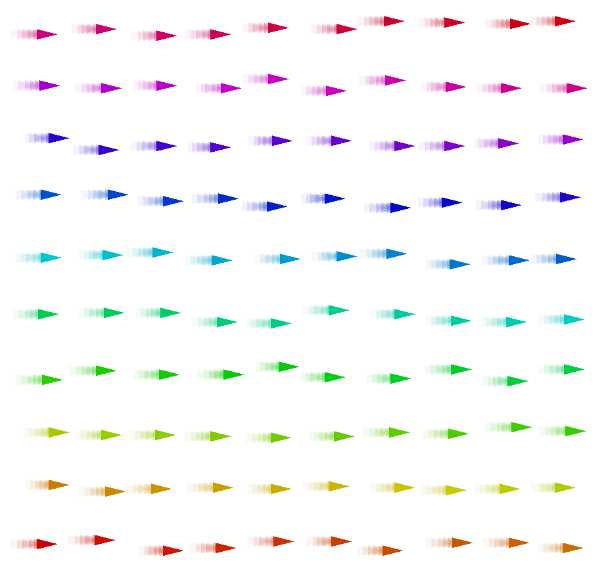
\includegraphics[height=3.5cm]{img/constant-movement.png}
		\end{exampleblock}
	\end{column}
	\begin{column}[t]{0.3\textwidth}
		\begin{exampleblock}{Obstacle avoidance}
		\begin{minted}{scala}
obstacleAvoidance(...)
		\end{minted}
		\centering
		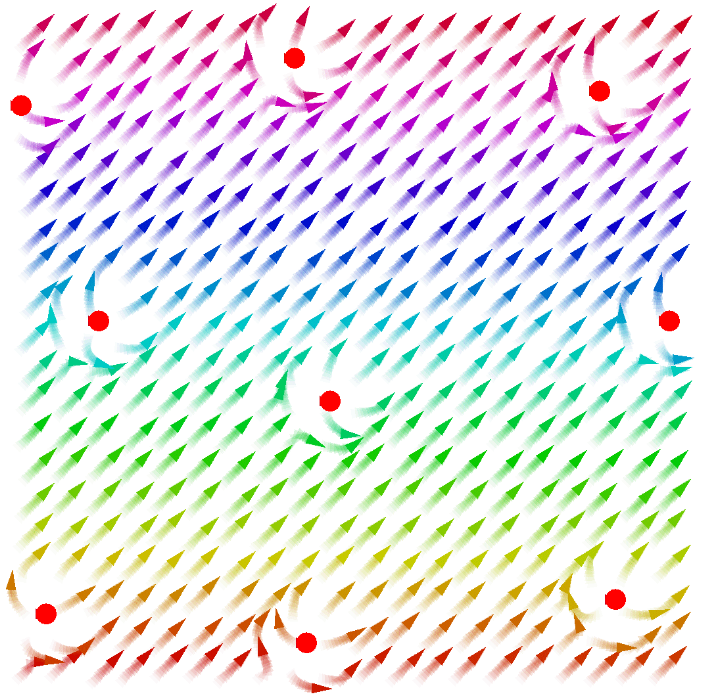
\includegraphics[height=3.5cm]{img/obstracle.png}
		
		\end{exampleblock}
	\end{column}
	\begin{column}[t]{0.3\textwidth}
		\begin{exampleblock}{Explore}
		\begin{minted}{scala}
explore(...)
		\end{minted}
		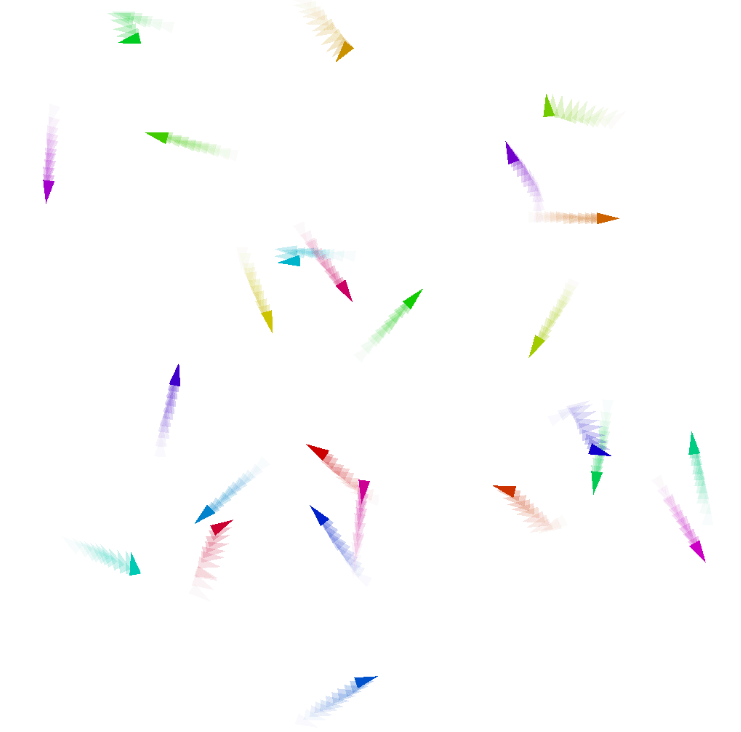
\includegraphics[height=3.5cm]{img/explore-2.png}
		\end{exampleblock}
	\end{column}
\end{columns}
\end{frame}
\begin{frame}[fragile]{API Overview}
\begin{columns}
\begin{column}{0.31\textwidth}
\begin{exampleblock}{Flocking\emph{\tiny{~\cite{reynolds1987flocks}}}}
\begin{minted}{scala}
rep(Zero)(v => reynold(v, ...))
\end{minted}
\centering
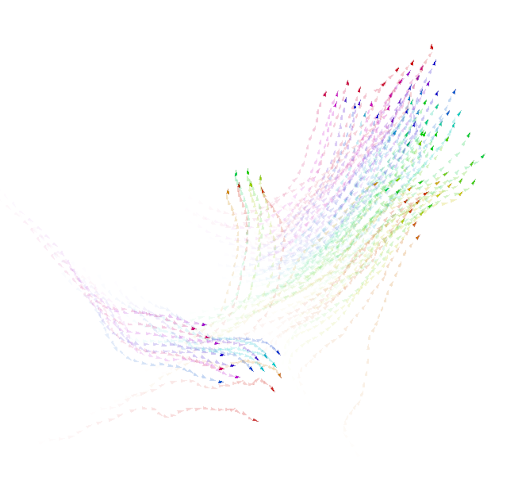
\includegraphics[width=0.8\textwidth]{img/flock.png}
\end{exampleblock}

\end{column}

\begin{column}{0.31\textwidth}
	\begin{exampleblock}{Leader Based\emph{\tiny{~\cite{DBLP:journals/tcst/GuW09}}}}
	\begin{minted}[fontsize=\scriptsize]{scala}
sinkAt(leader) // boolean field
	\end{minted}
	\centering
	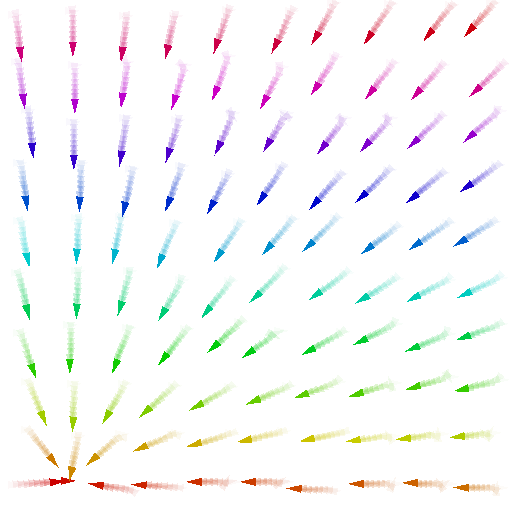
\includegraphics[width=0.8\textwidth]{img/towards-leader.png}
	\end{exampleblock}
\end{column}

\begin{column}{0.31\textwidth}
	\begin{exampleblock}{Team Formation}

\begin{minted}[fontsize=\scriptsize]{scala}
teamFormation(...)
\end{minted}
	\centering
	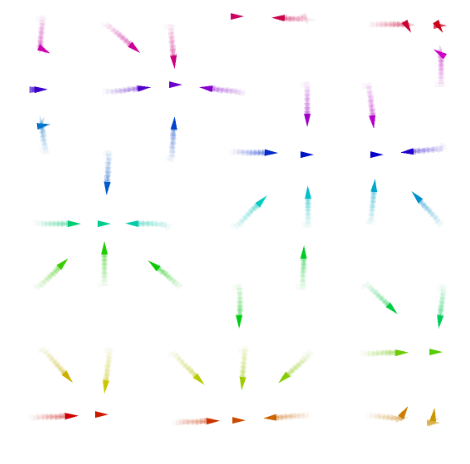
\includegraphics[width=0.8\textwidth]{img/team-formation-base.png}
	\end{exampleblock}
\end{column}
	
\end{columns}
\begin{exampleblock}{Pattern Formation\emph{\tiny{~\cite{DBLP:journals/ras/OhSSJ17}}}}
\centering
\texttt{line(...) || vShape(....) || centeredCircle(...)}

\includegraphics[width=0.8\textwidth]{img/shapes.png}
\end{exampleblock}
\end{frame}
%\begin{frame}{API Overview: Flocking}
%\centering
%Enable system-wide emergent behaviours of flocks of agents
%\end{frame}

%\begin{frame}{API Overview: Leader-based motion}
%	Allow the agents to follow a leader 
%	\centering
%\end{frame}
%\begin{frame}{API Overview: Team Formation}
%	\centering
%	Creation of groups of agents with different roles/tasks coordinated by a leader
%\end{frame}
\begin{frame}[fragile]{API Overview: Swarm Planning}

	Expressing a series of plans that change over time that let the swarm achieving different goals
\vspace{0.4cm}
\begin{columns}
\begin{column}{0.2\textwidth}
\centering
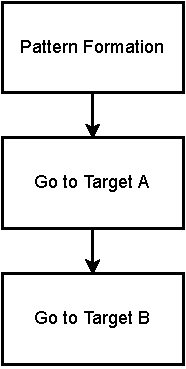
\includegraphics[width=\textwidth]{img/swarm-planner.drawio.pdf}
\end{column}
\begin{column}{0.3\textwidth}
	\begin{minted}{scala}
execute.once(
	plan {
		sinkAt(leader)
	}.endWhen {
		isTeamFormed(...)
	},
	plan(goToTop).endWhen {
		broadcast(leader, isClose(targetA))
	},
	plan(goToBottom).endWhen {
		broadcast(leader, isClose(targetB))
	}
)
	\end{minted}
\end{column}
\begin{column}{0.3\textwidth}
\centering
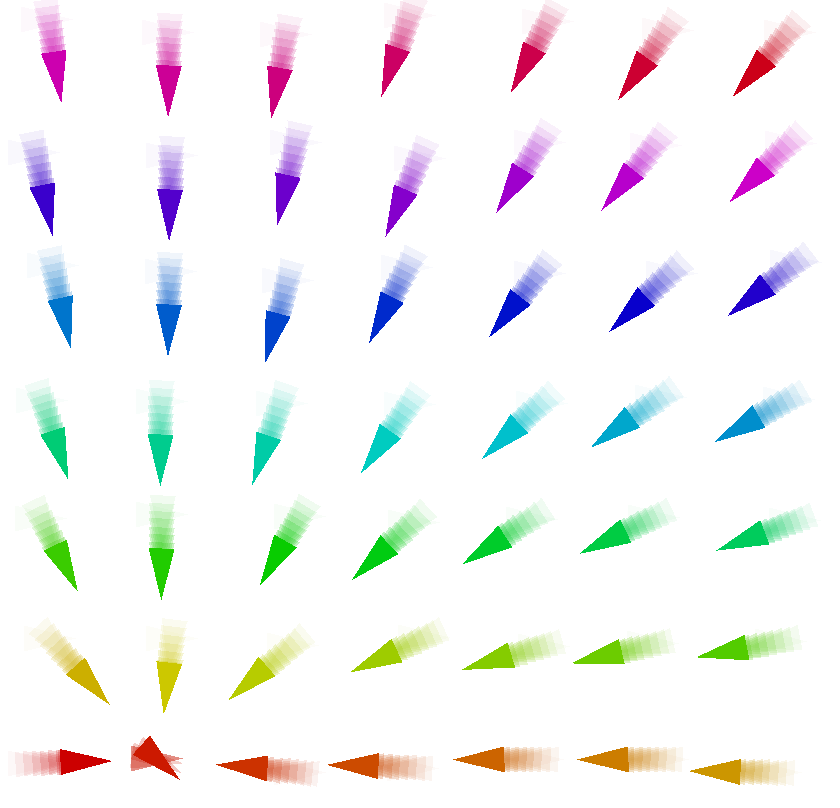
\includegraphics[width=0.5\textwidth]{img/go-to.png}

\includegraphics[width=0.5\textwidth]{img/go-to-1.png}

\includegraphics[width=0.5\textwidth]{img/go-to-2.png}
\end{column}

\end{columns}

\end{frame}

\begin{frame}[fragile]{API Overview: Composition}
The behaviours can be composed together to create more complex behaviours
\vspace{0.4cm}
\begin{columns}
\begin{column}{0.3\textwidth}
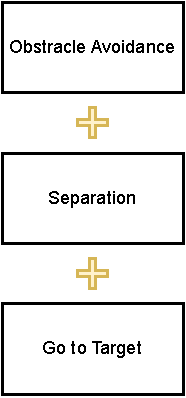
\includegraphics[width=0.7\textwidth]{img/swarm-composition.drawio.pdf}
\end{column}

\begin{column}{0.6\textwidth}
	\begin{minted}{scala}
val avoid = obstacleAvoidance(...)
val separation = separation(...)
val moveTo = goTo(target)
avoid + separation + moveTo
			\end{minted}
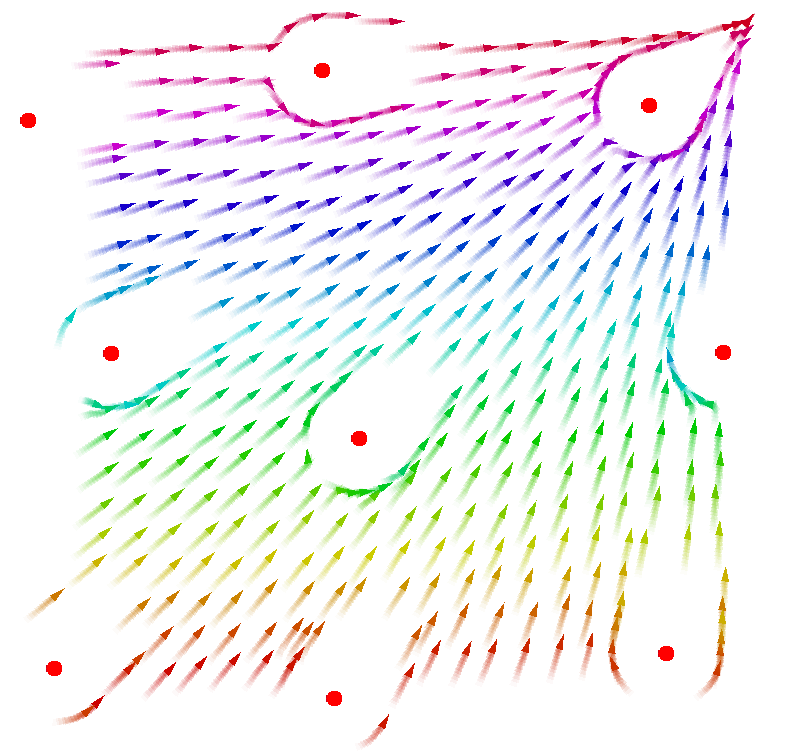
\includegraphics[width=0.7\textwidth]{img/composition.png}
\end{column}

\end{columns}
\end{frame}
\begin{frame}[fragile]{Use case: Rescue and Exploration}
\begin{exampleblock}{High-level description}
	\begin{itemize}
		\item A swarm of robots is deployed in a rectangular area in which there are injured target
		\item Two robots type: \emph{healers} and \emph{explorers}
		\item \textbf{Goal}: heal all the injured robots
		\item \url{https://github.com/AggregateComputing/experiment-2023-coordination-swarm-behaviour}
	\end{itemize}
\end{exampleblock}
\begin{columns}
\begin{column}{0.4\textwidth}

\begin{alertblock}{Pseudocode}
	\begin{enumerate}
		\item Form teams of robots with healers and explorers (\emph{team formation})
		\item Explore the area (\emph{exploration})
		\item When a robot finds an injured, it broadcasts a message (\emph{leader-based})
		\item The healers move towards the injured
	\end{enumerate}
\end{alertblock}
\end{column}

\begin{column}{0.55\textwidth}
	\begin{block}{MacroSwarm implementation}
		\begin{minted}[fontsize=\small]{scala}
execute.repeat(
	plan(formation(lead))
		.endWhen(circleIsFormed),
	plan(wanderInFormation(lead))
		.endWhen(dangerFound),
	plan(goToHealInFormation(lead, inDanger))
			.endWhen(dangerReached),
	plan(heal(healerId, inDanger))
)
		\end{minted}
	\end{block}
\end{column}

\end{columns}
\end{frame}
\begin{frame}{Use case: Results}
\centering
\fbox{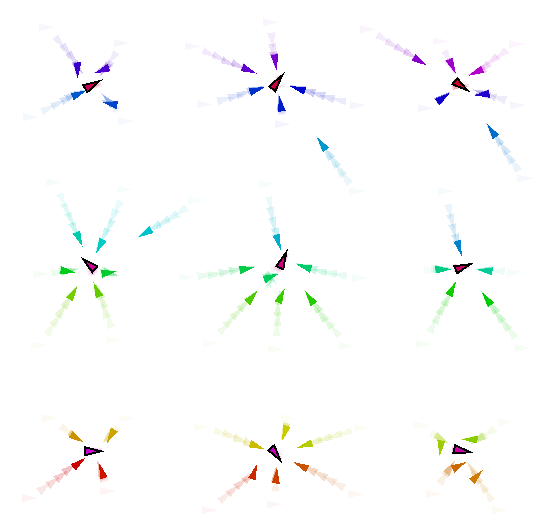
\includegraphics[height=2.3cm]{img/team-formation.png}}
\fbox{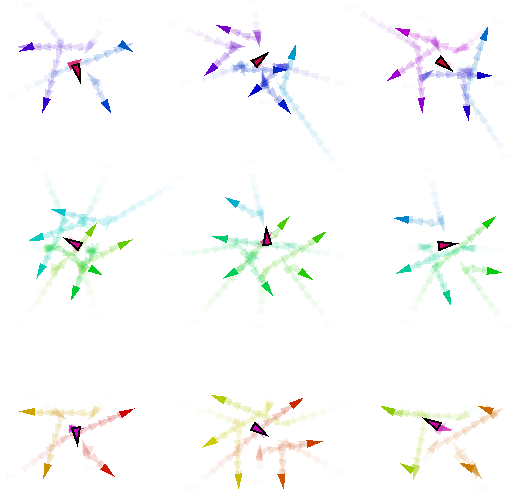
\includegraphics[height=2.3cm]{img/circle-formation.png}}
\fbox{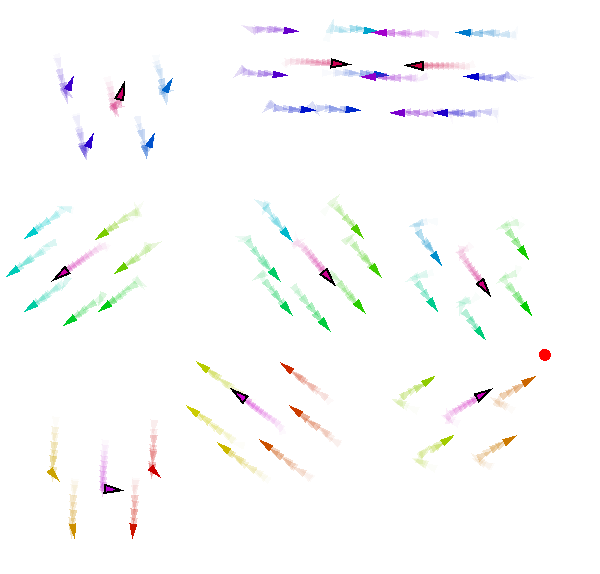
\includegraphics[height=2.3cm]{img/explore-append.png}}
\\
\vspace{0.1cm}
\fbox{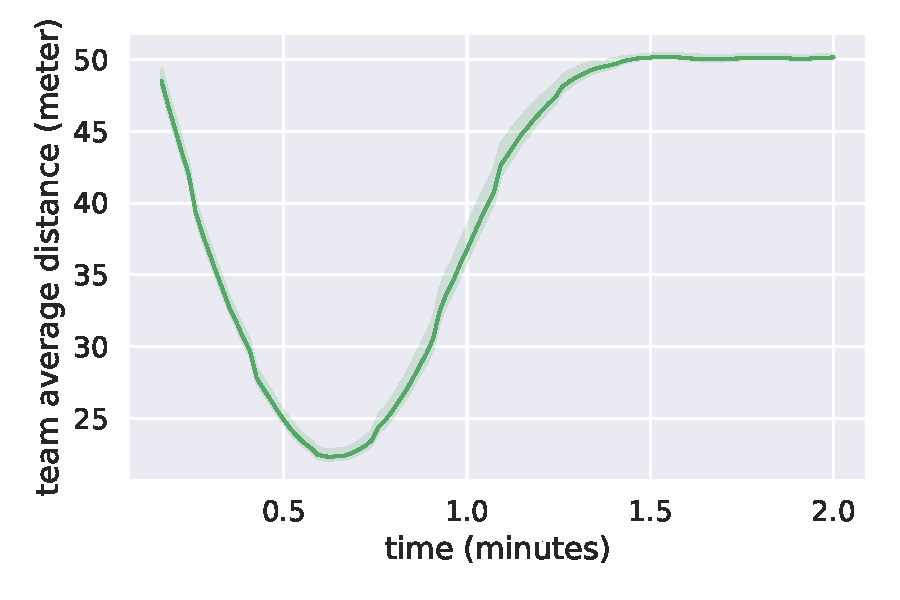
\includegraphics[width=0.3\textwidth]{img/average_intra_team_distance.pdf}}
\fbox{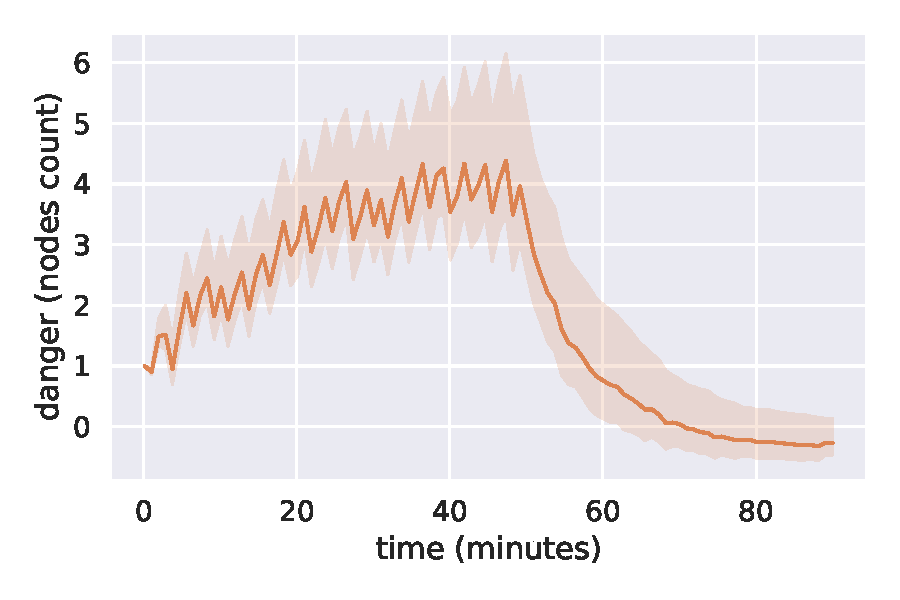
\includegraphics[width=0.3\textwidth]{img/in_danger.pdf}}
\fbox{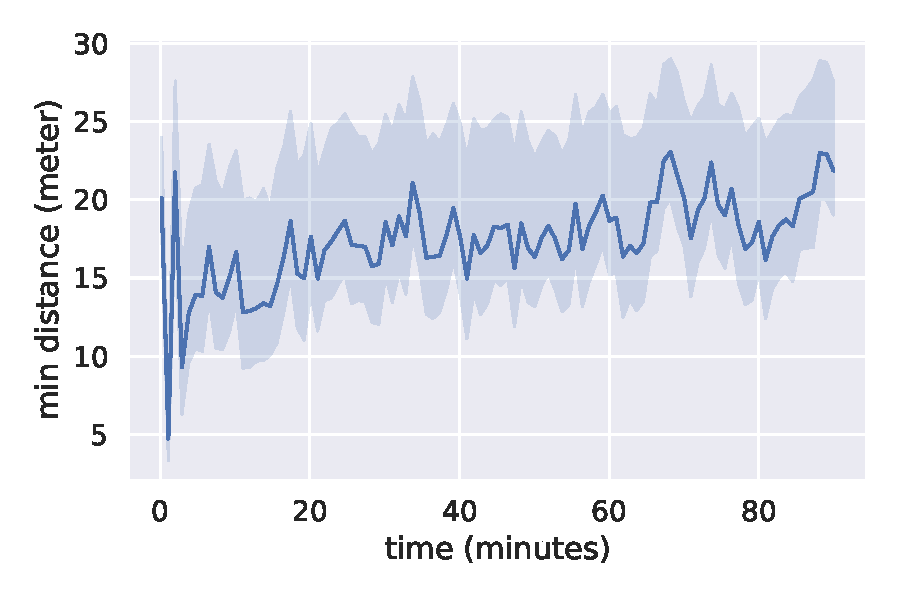
\includegraphics[width=0.3\textwidth]{img/min_distance.pdf}}
\begin{exampleblock}{}
	\begin{itemize}
		\item The swarm is able to form teams with the right shape (left figure)
		\item The swarm eventually solve the task (center figure)
		\item They avoid collisions (right figure)
	\end{itemize}
\end{exampleblock}
\end{frame}
\begin{frame}{Conclusion}
	\begin{exampleblock}{Wrap up}
		\begin{itemize}
			\item MacroSwarm: a new programming API for swarm robotics
			\item API overview covering main swarm behaviours
			\item Use case to exemplify the API usage
		\end{itemize}
	\end{exampleblock}
	
	\begin{alertblock}{Future work}
		\begin{itemize}
			\item Integration in a robust swarm robotics framework (e.g., ARGoS, Gazebo)
			\item Use in a real swarm of robots (e.g., using Crazyflie 2.0)
			\item Add more behaviours to the API (e.g., complex structures, easier plan composition)
		\end{itemize}
	\end{alertblock}
\end{frame}

\begin{frame}{}
\centering
\huge{Thank you for your attention!}
\\
\vspace{0.2cm}
\fbox{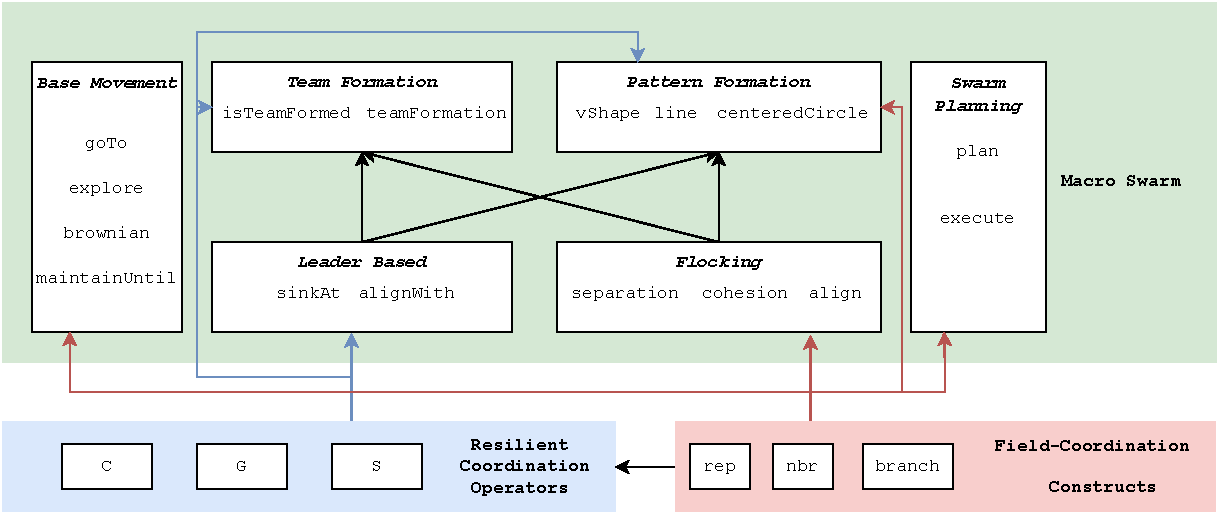
\includegraphics[width=0.5\textwidth]{img/architecture.drawio.pdf}}
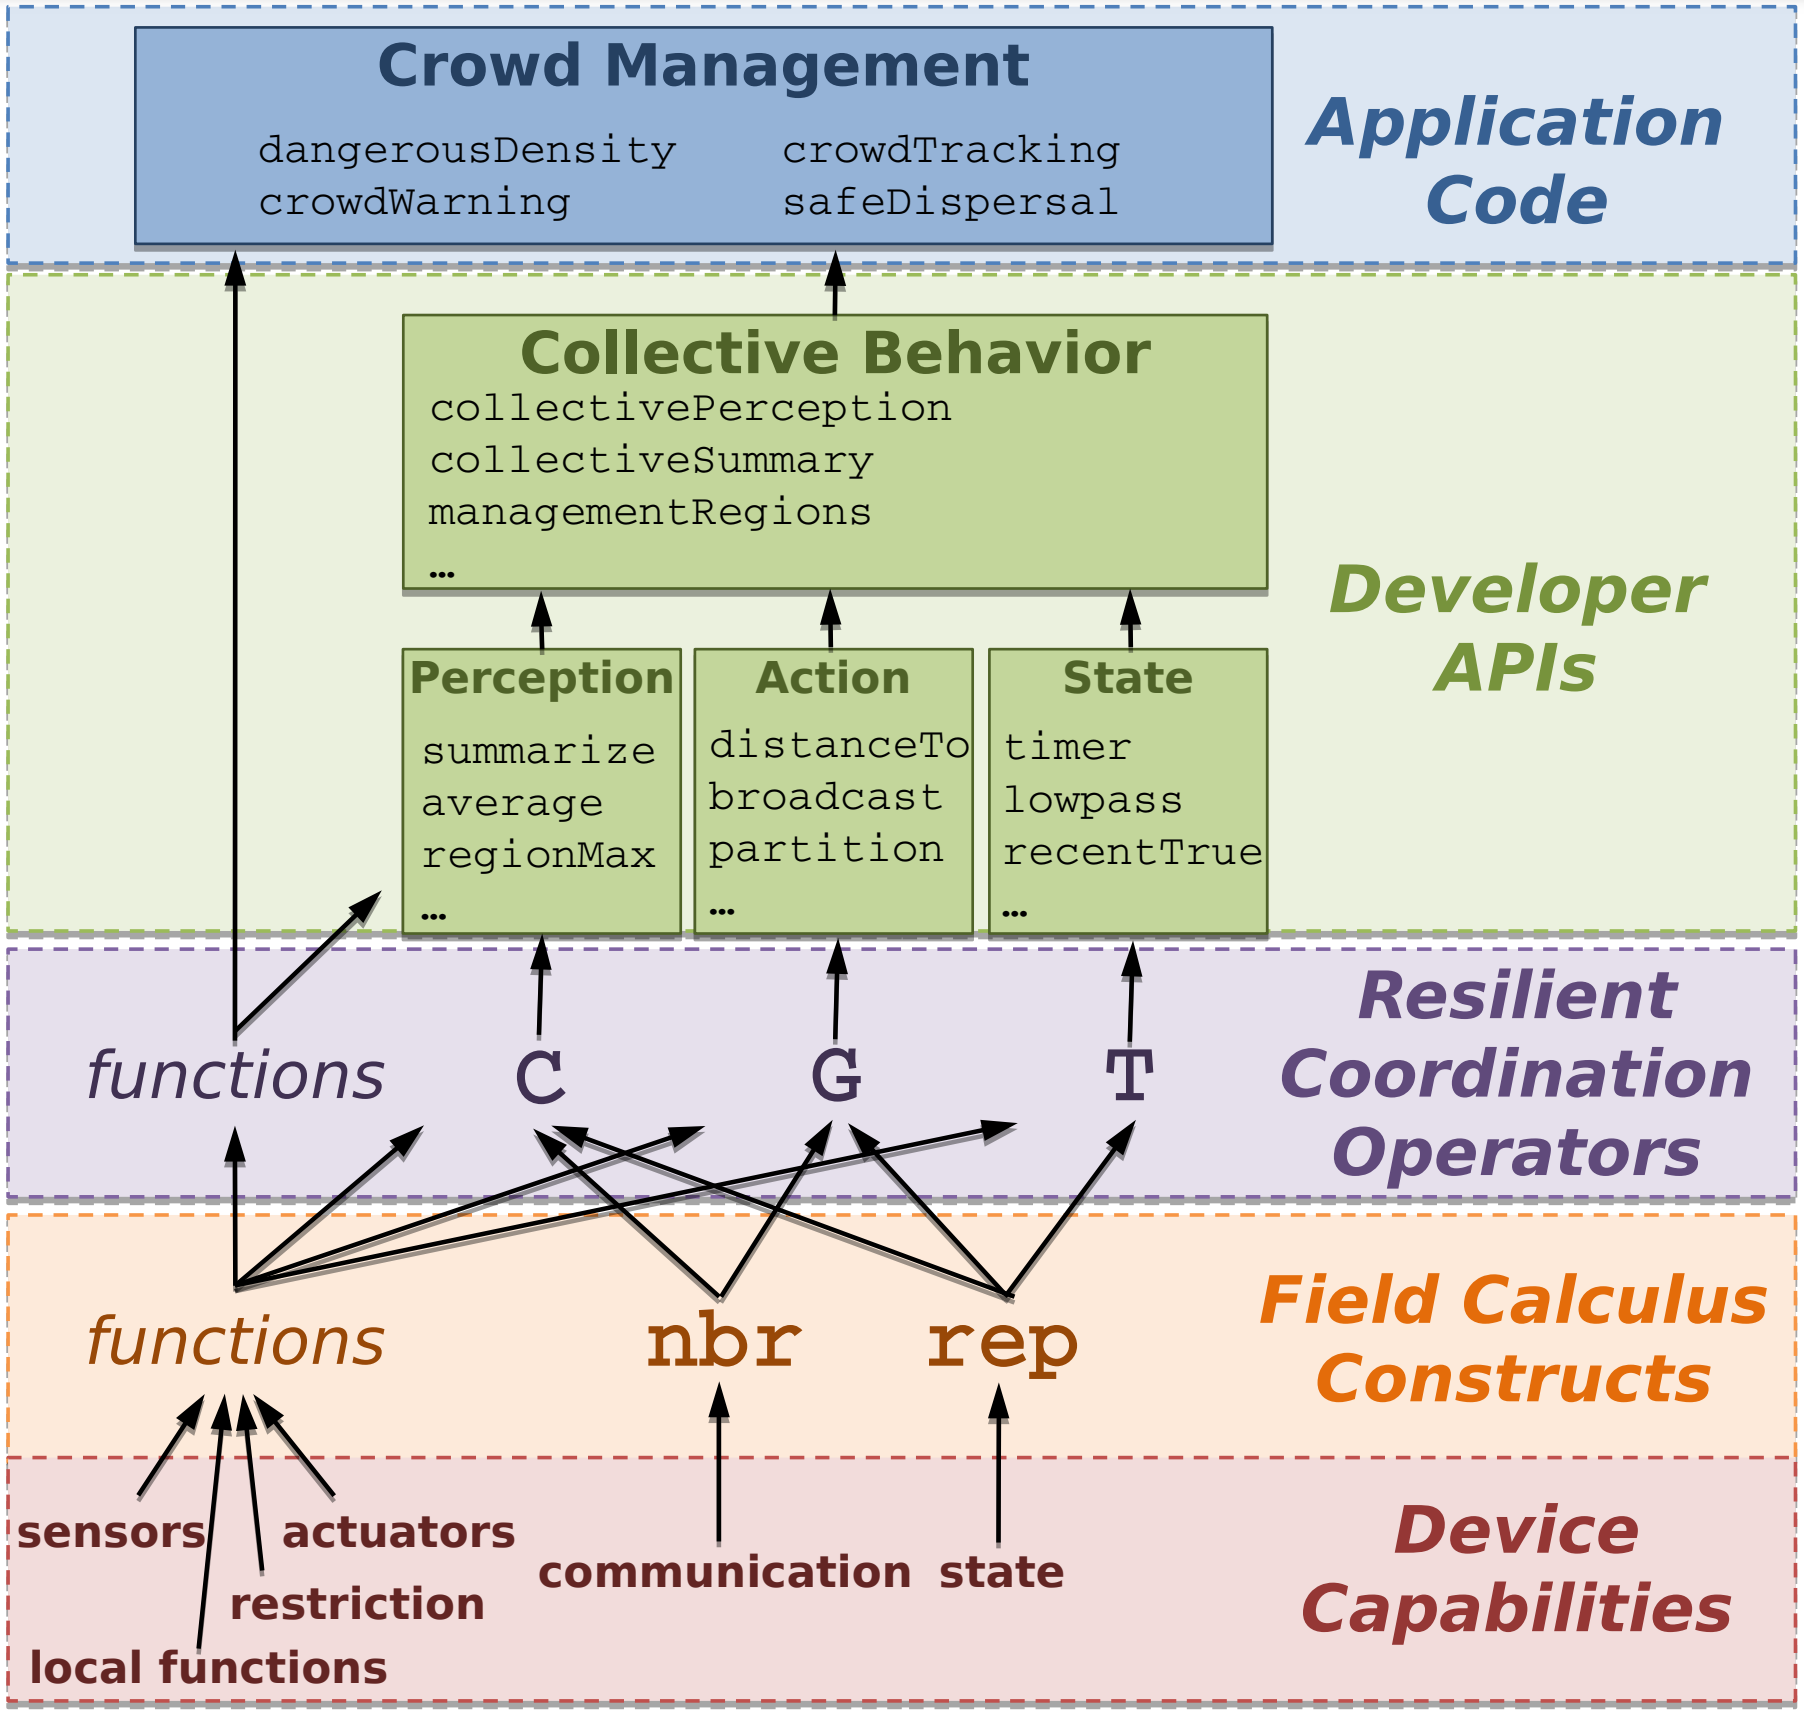
\includegraphics[height=2.8cm]{img/full-stack.png}
\\
\vspace{0.2cm}
\fbox{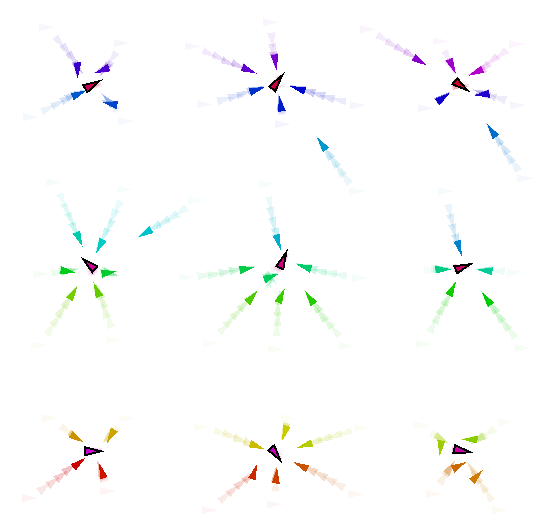
\includegraphics[width=0.2\textwidth]{img/team-formation.png}}
\fbox{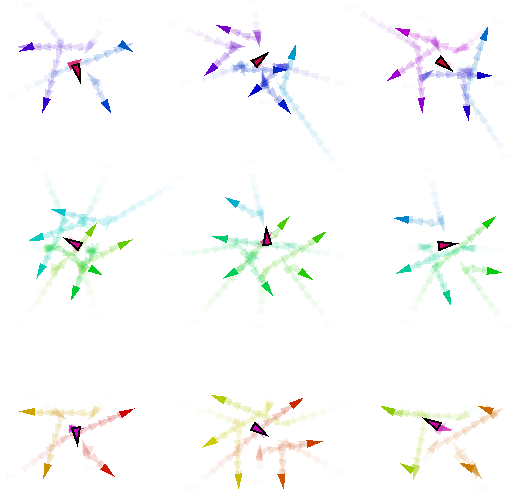
\includegraphics[width=0.2\textwidth]{img/circle-formation.png}}
\fbox{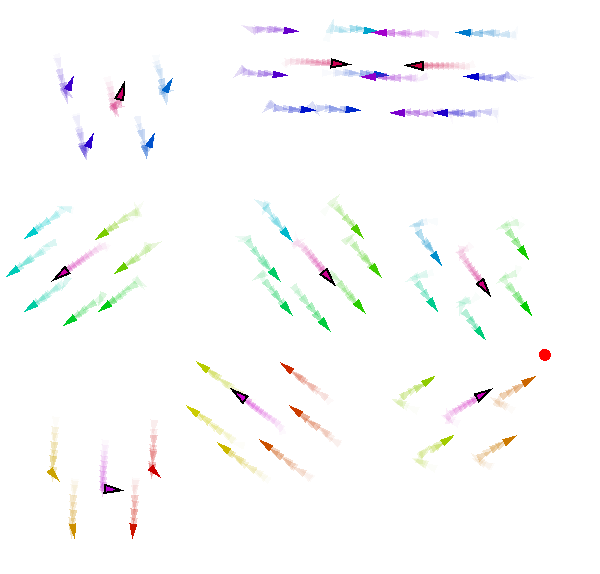
\includegraphics[width=0.205\textwidth]{img/explore-append.png}}
\\
\vspace{0.2cm}
\fbox{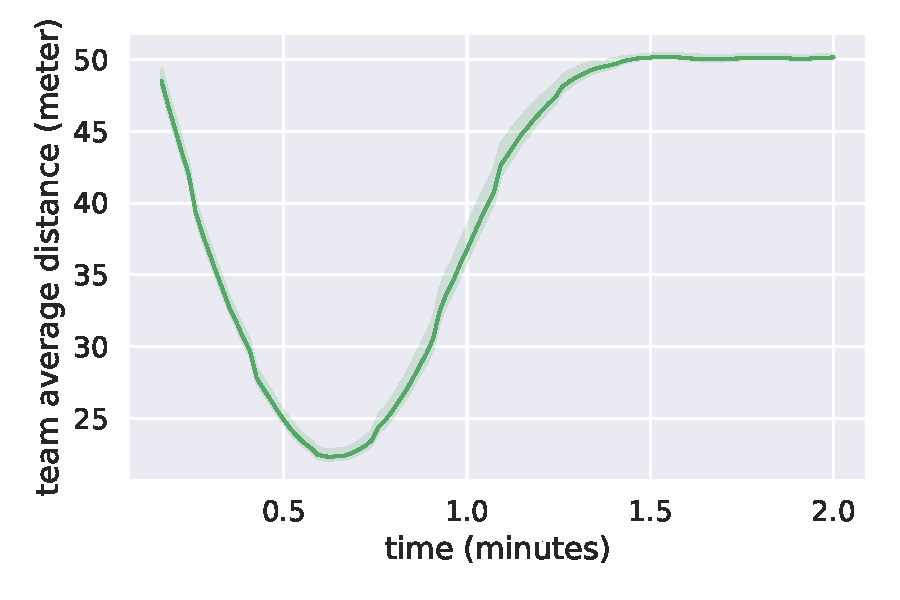
\includegraphics[width=0.2\textwidth]{img/average_intra_team_distance.pdf}}
\fbox{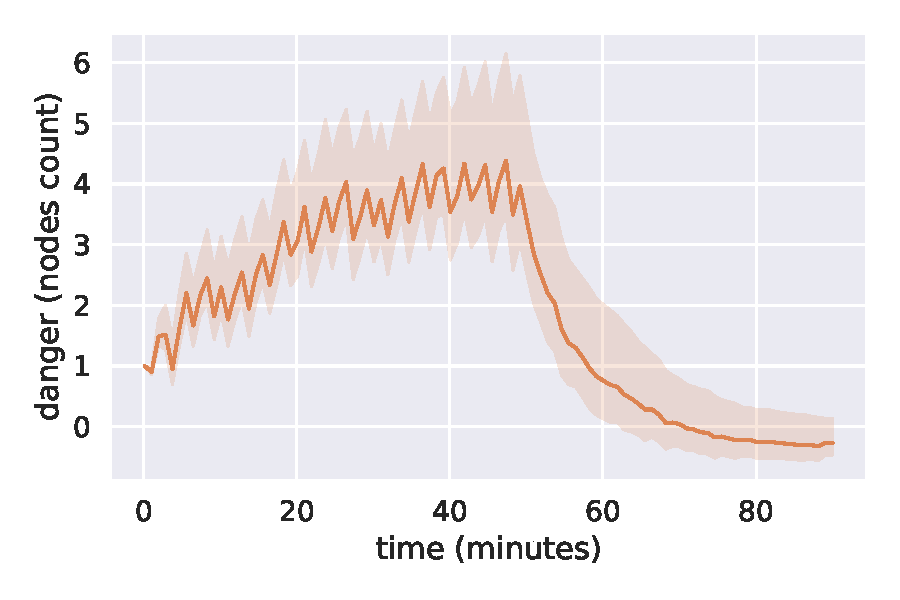
\includegraphics[width=0.2\textwidth]{img/in_danger.pdf}}
\fbox{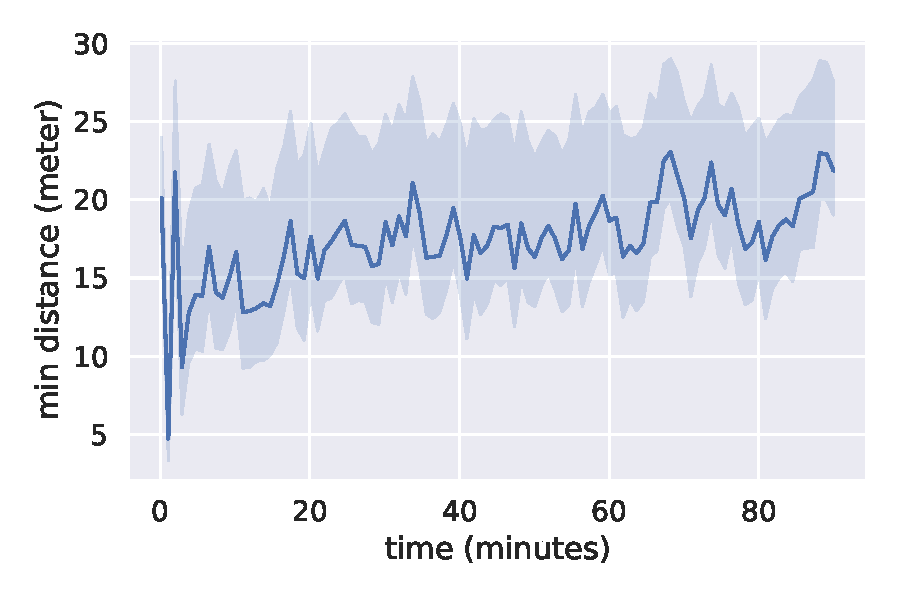
\includegraphics[width=0.2\textwidth]{img/min_distance.pdf}}
\end{frame}
%===============================================================================
\section*{}
%===============================================================================

%/////////
\frame{\titlepage}
%/////////

%===============================================================================
\section*{\refname}
%===============================================================================

%%%%
\setbeamertemplate{page number in head/foot}{}
%/////////
\begin{frame}[c,noframenumbering, allowframebreaks]{\refname}
%\begin{frame}[t,allowframebreaks,noframenumbering]{\refname}
	\tiny
	\printbibliography
\end{frame}
%/////////

%%%%%%%%%%%%%%%%%%%%%%%%%%%%%%%%%%%%%%%%%%%%%%%%%%%%%%%%%%%%%%%%%%%%%%%%%%%%%%%%
\end{document}
%%%%%%%%%%%%%%%%%%%%%%%%%%%%%%%%%%%%%%%%%%%%%%%%%%%%%%%%%%%%%%%%%%%%%%%%%%%%%%%%
